% HCI Group Konstanz Seminar Template
%
% ATTENTION: This template was designed to fit the most common requirements for different types of reports (e.g., Seminar to the Project or Project Report). However, if you feel the need to add an extra component or layout feature please talk to your advisor. Please do not change anything on this template unless it is explicitly allowed or agreed with your advisor. However, it is allowed to add packages that do not alter the design/layout of this template.
%

\documentclass[10pt, paper=a4, parskip, oneside]{scrreprt}
\usepackage[T1]{fontenc}
\usepackage[utf8]{inputenc}
\usepackage{hciknseminar}
\usepackage[ngerman, english]{babel} % Spell checking (Using ngerman for german spell checking). The last language is the standard language for the document.
\usepackage{enumitem}

\bibliography{bibliography} % Reference to bibliography.bib file

% ============= Commands =============
\newcommand{\exgo}{E(x$\mid$g)o}
\newcommand{\todo}[1]{\textcolor{red}{todo: #1}}

\usepackage{float} % for H, remove of anything breaks
% ============= Abstract =============
\abstract{
Motor Learning in Mixed Reality prooved to be good. But view reseach in the influence of the perspective on guidance visualisation. This work proposes a study to investigate this. Task is handling physical load. will enable designers of MR ML systems to base their work on on empirical data.
}

% ============= Document =============
\begin{document}
	% =========== Title page ============
	\begin{titlepage}
		\begin{center}
			{\LARGE \textbf{Ego OR Exo:\\Comparing Visual Perspectives on Guidance Visualisations for Motor Learning}}
			\\[1cm]
			{\Large \textbf{Masterarbeit}}
			\\[1cm]
			{\Large vorgelegt von}
			\\[0.5cm]
			{\LARGE \textbf{Stefan Paul Feyer}}
			\\[0.5cm]
			{\Large an der}
			\\[0.5cm]
			
\includegraphics[width=0.4\textwidth]{figures/unisignet.pdf}
			\\[1cm]
			{\Large \textbf{Sektion Mathematik und Naturwissenschaft}}
			\\[1cm]
			{\Large \textbf{Fachbereich Informatik und Informationswissenschaft}}
			\\[2cm]
			\begin{minipage}[c]{0.8\textwidth}
				\begin{description}[style=multiline]
					\item {\Large \textbf{1.Gutachter:} Prof. Dr. Harald Reiterer}
					\item {\Large \textbf{2.Gutachter:} Dr. Karsten Klein}
				\end{description}
			\end{minipage}
			\vfill
			{\LARGE \textbf{Konstanz, 2021}}
		\end{center}
	\end{titlepage}

% Abstract
\makeabstract
% Table of contents
\tableofcontents
\addcontentsline{toc}{chapter}{Contents} % Add contents to table of contents
% List of Figures
\listoffigures
\addcontentsline{toc}{chapter}{\listfigurename} % Add list of figures to table of contents
% List of Tables
\listoftables
\addcontentsline{toc}{chapter}{\listtablename} % Add list of tables to table of contents
% Prepare chapters
\clearpage
\setcounter{romanPages}{\value{page}} % Update variable for roman pages
\pagenumbering{arabic} % Turn on page numbering again

\chapter{Introduction}
The acquisition of movements is a crucial part of human development\cite{mlbook}. Learning movements empowers to be more efficient, faster or more exact (ibid.) for tasks like sports, arts or the ergonomic handling of physical load. The process of learning movements is called motor learning.\\
Movements can be learned by voyeurism and mimicking: watching and trying it out by oneself. Mastering a movement mostly includes an experienced teacher. A teacher is hardly replaceable because of immediate visual, audible and haptic feedback on a movement performed. However, if a teacher is not available, for example, based on the location or economic reasons, other sources can be used to learn movements. For example, YouTube\footnote{\href{https://www.youtube.com/}{https://www.youtube.com/}, accessed 17.2.2021} and other video platforms have become a great source for learning videos for a wide range of purposes. The downside of video recordings is the two dimensional (2D) experience of a three dimensional (3D) movement. Mixed Reality devices can transport the learning process into the digital world. In contrast to video recordings, Mixed Reality can provide the learning experience in 3D. Furthermore, Mixed Reality can provide feedback on the performed movement and has the ability for interactions with the virtual guidance visualisation. Mixed Reality has already proven to be a suitable environment for motor learning for tasks like dancing~\cite{YouMove,vrdancetrainer,outsideme,performancetraining,mrdancetrainer}, sports~\cite{freethrowsimulator,trainingphysicalskills}, rehabilitation~\cite{motionma,physioathome,kinohaptics,sleevear,veimprovesml}, arts~\cite{ararm,justfollowme,stylo,elearningma,mythaichicoaches,rtgesturerecognistion,onebody,thaichichua} and others~\cite{tikl,lightguide}. However, this master's thesis will focus on Virtual Reality.\\
In the real world, where the learner and teacher are real persons, the learner sees the teacher, for example, in front of himself/herself. This perspective is called the exo-centric visual perspective. Nevertheless, if we move from the real world to the virtual world of Virtual Reality, we are no longer restricted to the exo-centric visual perspective. The teacher can be rendered inside the learners' body, allowing the learner to see the teacher from an ego-centric perspective. The change from the exo-centric to the ego-centric visual perspective potentially influences motor learning, which is shown by previous research. For example, AR-Arm~\cite{ararm} lets the learner experience the movements from an ego-centric perspective. YouMove~\cite{YouMove} teaches dance from an exo-centric perspective. OneBody~\cite{onebody}, LightGuide~\cite{lightguide}, Mixed Reality Dance Trainer~\cite{mrdancetrainer}, Free Throw Simulator~\cite{freethrowsimulator}, Training Physical Skills~\cite{trainingphysicalskills}, Sleeve AR~\cite{sleevear} and Tai Chi Trainer~\cite{thaichichua} use both visual perspectives or a combination of them. However, only OneBody, LightGuide and Tai Chi Trainer found differences between the visual perspectives.\\
Another topic where Virtual Reality could be a valuable helper is the ergonomic conduction of movements while handling physical loads~\cite{nursecare,kitt}. The handling of physical load is part of working routines and everyday life. Handling physical load in the correct ergonomic conduct in working routines can prevent injuries in everyday life. However, a kinaesthetics teacher is not always accessible, for example, for economic reasons. The influence of the visual perspective on a virtual guidance visualisation teaching the handling of physical load in Virtual Reality is sparsely investigated. Especially, locomotion movements like walking or carrying in the ego-centric perspective are left out. The lack of research on the influence of the visual perspective on a virtual guidance visualisation, especially for handling physical loads, shows the necessity of investigations on:
\begin{itemize}
	\item[RQ1:] How does the visual perspective on a virtual guidance visualisation influence motor learning in Virtual Reality environments?
\end{itemize}
To answer this main research question RQ1, several aspects have to be taken into account: accuracy of movements, transfer of information about how to move, the visual focus of the learner, and last but not least, the personal preference of the learner. Therefore, to answer the main research question RQ1, it is necessary to answer the following sub-research questions:
\begin{enumerate}[align=left, leftmargin=0pt, labelindent=\parindent,
	listparindent=\parindent, labelwidth=0pt, itemindent=!]
	\item[RQ1.1] How does the visual perspective on a virtual guidance visualisation influence movements' accuracy?
	\begin{itemize}
		\item[] \begin{itemize}
			\item[RQ1.1.1] How does the visual perspective on a virtual guidance visualisation influence movements' accuracy of the own body?
			\item[RQ1.1.2] How does the visual perspective on a virtual guidance visualisation influence the accuracy of handling physical load?
			\item[RQ1.1.3] How does the visual perspective on a virtual guidance visualisation influence subtasks' accuracy?
		\end{itemize}
	\end{itemize}
	
	\item[RQ1.2] Does the visual perspective on a virtual guidance visualisation influence the transfer of ergonomic principles?
	\item[RQ1.3] How does the visual perspective on a virtual guidance visualisation influence the learner's visual focus?
	\item[RQ1.4] What is the subjective personal preference of the learner for the visual perspectives?
\end{enumerate}
The answers to these research questions will enable designers of Virtual Reality motor learning training systems to choose a suitable visual perspective on an empirical basis.

\section{Outline}
This master's thesis aims to increase the empirical evidence of how the visual perspective influences motor learning in Virtual Reality by proposing an experiment. This document will present the development of an experiment and a system with which the experiment can produce this data.\\
First, the theoretical foundations are laid out, and a state-of-the-art analysis on the basis of related work is provided in chapter~\ref{chapter:theoretical_background}. With the fundamentals at hand, chapter~\ref{chapter:studysetting_conduction} describes in detailed the design of the proposed experiment. Chapter~\ref{chapter:studysetting_conduction} will adress the independent variables (\ref{sec:visualPerspecticves}) and dependent variables (\ref{sec:measures}) of the experiment as well the task design (\ref{sec:taskDesign}).\\
To conduct the experiment, a system was implemented that fulfils the needs of the experiment. This system is called \exgo. The design and implementation of \exgo\ is pictured in chapter~\ref{chapter:system}. The experiment requires a digital representation of the learner (\ref{sec:selfperception}) and the guidance visualisation (\ref{sec:gv}). Furthermore, physical and digital artefacts the learner will interact with need to be constructed and built physically and digitally (\ref{sec:artefacts}). The digital representations of learner and guidance visualisation as well as the artefacts are then arranged to form the visual perspectives (\ref{sec:perspectives}). Subsequently, the acquisition of the quantitative (\ref{sec:logging}) and qualitative (\ref{sec:quali_logging}) data is described. Finally, the elements of the experiment design and \exgo\ are composed, and an experiment procedure is defined (\ref{sec:procedure}). The experiment was evaluated by a pilot study, the results and possible improvements are shown in chapter~\ref{chapter:study_evaluation}. In the end, this master's thesis closes with a conclusion and outlook in chapter~\ref{chapter:conclusion}. The appendix provides a Glossarium, additional figures and the experiment's documents.



%This work proposes a study design to answer the research question. To design this study on a solid basis, the theoretical foundations a laid in chapter~\ref{chapter:theoretical_background} with a closer look on Motor Learning (section~\ref{section:motor_learning}), visual perspectives (section~\ref{section:visual_perspectives}) and Mixed Reality (section \ref{section:mixed_reality}). These sections result in the scope and parameters of the study design. Section~\ref{section:related_work} investigates previous works and illustrates the conceptual delimitation of this work from what has already been investigated. Chapter~\ref{chapter:theoretical_background} concludes with a research contribution statement, clarifying the Empirical Contribution and Artifact Contribution of this work.\\
%For the proposed study, a system had to be designed to produce data to answer the research questions. This system is called \exgo\. The design and implementation is described in section~\ref{section:system} followed by the design of the study itself in section~\ref{section:study}.\\
%\exgo\ and the study design have been evaluated in a pilot study. The results of the evaluation are depicted in chapter~\ref{chapter:study_evaluation}. Furthermore, this chapter suggests improvements in the study design in section~\ref{section:study_improvements}. This work concludes in chapter \ref{chapter:conclusion} with an outlook on how \exgo\ can be enhanced and expanded as well as used for further investigations.

%Motivation: Motorlearning wichtig zur aneignung von bewegungen. am besten mit echtem lehrer. wenn dieser nicht verfügbar, motor learning in VR möglich und sinnvoll, siehe xyz. allerdings ist der einfluss der perspektive auf die virtuelle guidance vis. noch wenig untersucht. deswegen diese arbeit hier.\\
%ferner, wenig motorlearning in zusammenhang mit physical load und wenig "laufen mit egozentrischer anleitung".\\
%Daraus folgt die forschungsfrage ... und ihre sub forschungsfragen ...\\
%Um daten zu generieren um diese forschungsfragen zu beantworten wurde Exgo entwickelt. Eine studie wurde designed um mit diesem system die notwendigen daten zu generieren.\\
%Diese arbeit beschreibt design und entwicklung von exgo, sowohl als auch die entwicklung dieser studie. EIn pilottest und dessen überarbeitung ist angeschlossen. auch weiter forschungsmöglichkeiten mit dem system sollen aufgezeigt werden.\\

\chapter{Motor Learning in Virtual Reality}
\label{chapter:theoretical_background}
This chapter provides the theoretical background of Virtual Reality, motor learning, Visual Perspectives, handling physical load and injury risk metrics in a condensed form. For a more detailed description of these topics, please refere to the preceeding seminar thesis~\cite{seminarThesis} which is also digitally attached to this master's thesis. These topics are the most important aspects that serve as the foundation for this master's thesis. Subsequently, an analysis of related work is provided. This chapter gives insights into how this work is informed and differentiated from other researchers. Finally, the research contribution statement is provided.

\section{Virtual Reality}
\label{section:mixed_reality}
\begin{figure}[H]
	\centering
	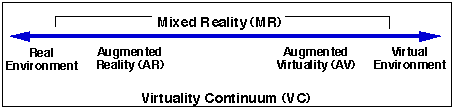
\includegraphics[width=\textwidth]{figures/milgram_continuum.png}
	\caption[Mixed Reality continuum by Milgram et al.]{Mixed Reality continuum by Milgram and Kishinho~\cite{mrcontinuum}}
	\label{fig:mrCont}
\end{figure}
Milgram and Kishinho~\cite{mrcontinuum} describe Mixed Reality (MR) for visual displays on a continuum, compare figure~\ref{fig:mrCont}. Virtual Reality (VR) is purely digital, and thereby the environment is blocked entirely. In Augmented Reality, the environment is visible and augmented with digital elements. During motor learning, the visual perception of one's own body is desirable, because it is the most exact representation of one's own body. Thereby, the approach of augmenting the real-world body with a virtual guidance visualisation (GV) is promising. However, today's AR-technology provides a small field of view. A solution to this could be the video see-through technology, but it is limited by latency and distortion~\cite{max}.\\
The body's perception can also be achieved by tracking the learner's body and render it over the learner's physical body. Though, the visual perception of the learner's body can be established in VR. Consequentially, this work will focus on motor learning in Virtual Reality.

\section{Motor Learning}
\label{section:motor_learning}
Motor learning is achieved through instruction, attempt, imitation or a combination of them~\cite{mlbook}. The process of motor learning can be divided into three parts: cognitive stage, associative stage and autonomous stage (ibid.). In the cognitive stage, training methods are most efficient, and the performance gain ist the highest among the stages (ibid.). Tasks that belong to this stage are thereby best suited for an experiment.\\
Movements can be classified by two means: by \textit{particular movements} and based on \textit{perceptual attributes} (ibid.). Based on the \textit{particular movements}, the classification is described by a continuum, compare figure~\ref{fig:movement_classification} left. On the extremes of the continuum are \textit{discrete movements} and \textit{continuous movements}. Between these extremes, \textit{serial movements} are located. \textit{Discrete movements} are too short for an evaluation. \textit{Continuous movements} do not have a recognisable beginning, and thereby they are not suitable for the experiment in question either. \textit{Serial movements} are chained \textit{discrete movements} with a recognisable beginning and end. This allows a task decomposition and an evaluation of particular subtasks. Furthermore, \textit{serial movements} are generally more complex than \textit{discrete} or \textit{continuous movements} and therefore more suited for movement training systems. \textit{Serial movements} are widely used for research in motor learning, for example~\cite{lightguide,mythaichicoaches,elearningma}. Therefore, the experiment task design of this master's thesis is based on \textit{discrete movements}.\\
The classification based on the \textit{perceptual attributes} is also represented by a continuum and includes the environment in which the movement is performed, compare figure~\ref{fig:movement_classification} right. At the extremes of the continuum, \textit{open skills} and \textit{closed skills} are located. For \textit{closed skills}, the environment is predictable, while for\textit{ open skills}, the environment is not predictable. The experiment aims to analyse the learners' performance of following a movement and not how they can adapt to environmental changes. Thereby, this experiments task for this master's thesis must be located on the left-hand side of the continuum: \textit{closed skills}.
\begin{figure}[htb]
	\centering
	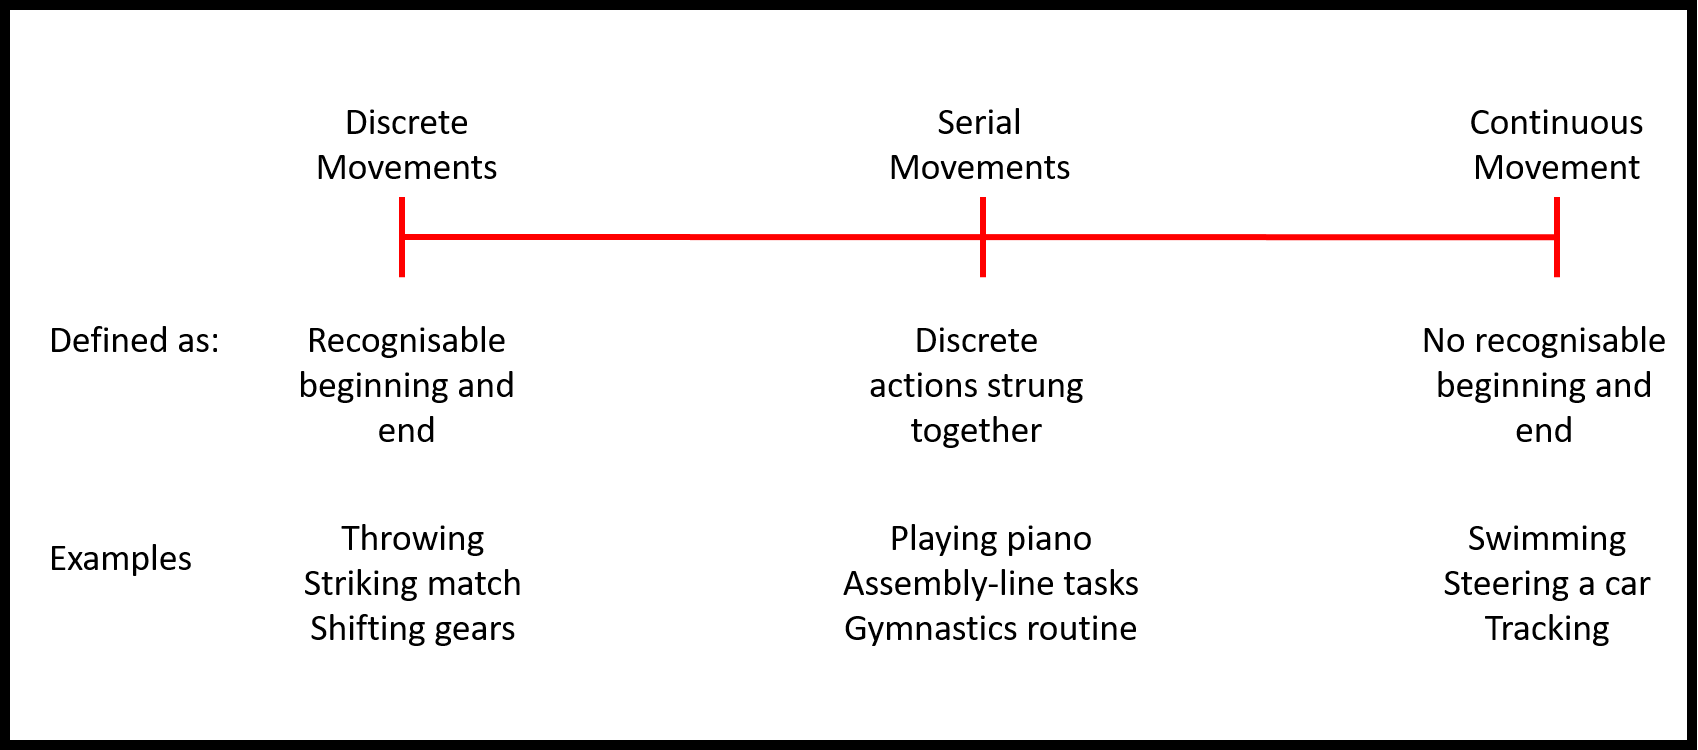
\includegraphics[width=0.49\textwidth]{figures/movement_classification.png}
	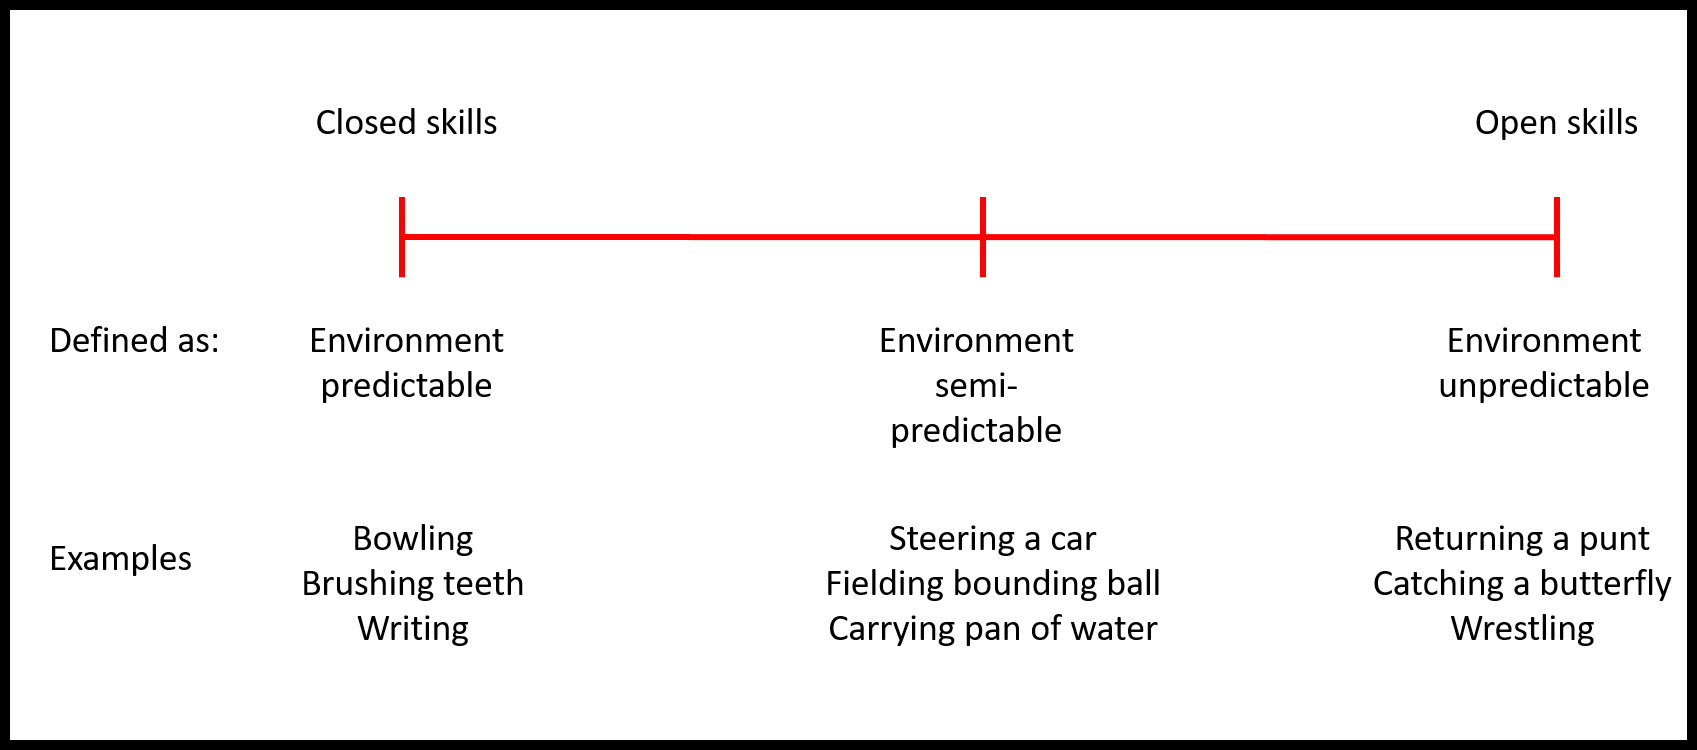
\includegraphics[width=0.49\textwidth]{figures/movement_classification2.png}
	\caption[Movement classifications by Scmhidt et al.]{Movement classification by \textit{particualar movement} (left) and \textit{perceptual attributes} by Schmidt et al.~\cite{mlbook}}
	\label{fig:movement_classification}
\end{figure}

\subsection{Measurements for Motor Learning}
\label{section:measures_for_ml}
The movements of a teacher and the movement of a learner differ. To assess the difference between the two movements, two main classes of measures can be applied~\cite{mlbook}: \textit{measures of error for a single object} and \textit{measures of time and speed}.
\textit{Measure of error for a single object} represent the degree to which the target movement is amiss. Schmidt et al.~\cite{mlbook} provide five \textit{error measures} to calculate this error. Among them, \textit{constant error} is the most common measure in related work to determine the difference between the movement of the learner and the movement of the teacher, for example~\cite{perspectivematters,thaichichua,YouMove,onebody,vrdancetrainer,lightguide,physioathome}. \textit{Constant Error} is defined as the average error between the learner's movment and the teacher's movement and is described as
\begin{equation}
	\label{eq:constanterror}
	CE=\frac{\sum_i(x_i-T)}{n}
\end{equation}
with $x_i$: actual value, $T$: target value, $n$: number of values~\cite{mlbook}.\\
The basic idea of \textit{measures of time and speed} is that a performer who can accomplish more in a given amount of time or who can accomplish a given amount of behaviours in less time is more skillful. In related work, this measure is mostly assessed by the task completion time, for example~\cite{perspectivematters,onebody,lightguide}.


\section{Visual Perspectives}
\label{section:visual_perspectives}
\begin{figure}[H]
	\centering
	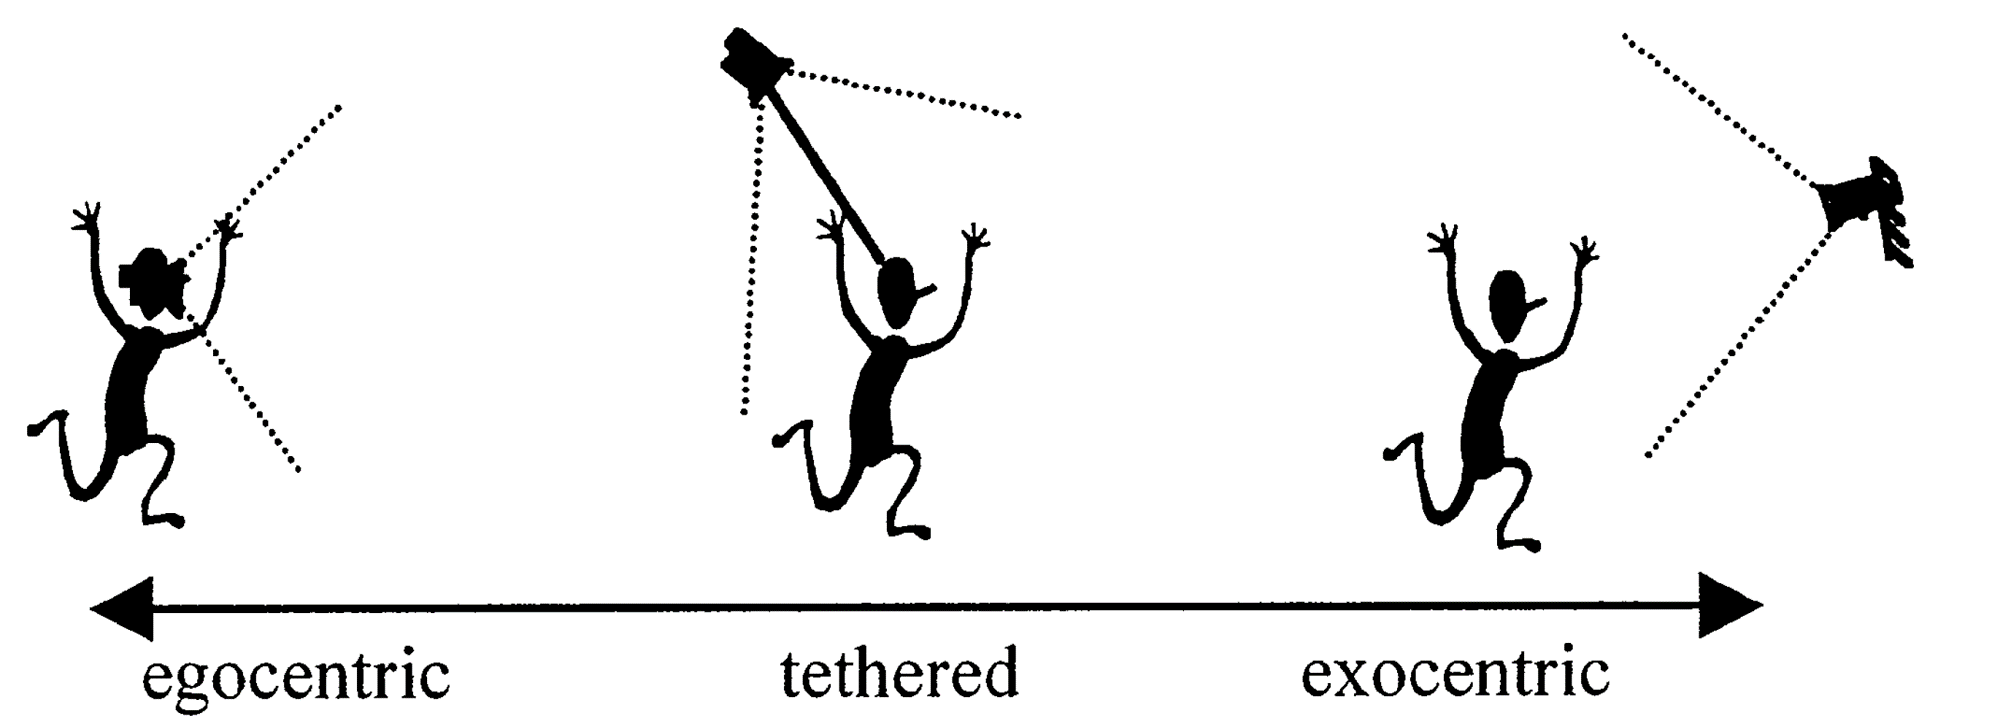
\includegraphics[width=\textwidth]{figures/ego_exo_continuum.PNG}
	\caption[Centricity continuum by Wang et al.]{Centricity continuum by Wang and Milgram~\cite{centricitycontinuum}}
	\label{fig:ego-exo-continuum}
\end{figure}
Wang and Milgram~\cite{centricitycontinuum} describe visual perspectives (VP) by the \textit{centricity continuum}, compare figure~\ref{fig:ego-exo-continuum}. On the left extreme on the continuum, the ego-centric VP is located, in literature also called first-person perspective (1PP). On the right extreme, is the exo-centric VP, in literature also called third-person perspective (3PP). The middle part represents tethered VP. By moving from the left to the right, the so-called \textit{tethering distance} increases. The \textit{tethering distance} describes the distance of the anchor point of the eyes to the object in question. In this master's thesis, the "object in question" is the human-shaped guidance visualisation (avatar). VPs can be clustered into three classes: ego-centric VPs (g-class), exo-centric VPs (x-class) and VPs that contain both ego-centric and exo-centric VPs (gx-class). Without the usage of additional perpsective influencing artefacts like mirrors, cameras or screens, there are five possible VPs:
\begin{itemize}
	\item \textbf{Ego-centric}: the teacher's avatar is located inside the learner's avatar. The learner sees the GV inside one's own body, compare figure~\ref{fig:perspectives} top left and figure~\ref{fig:ego}.
	\item \textbf{Purely exo-centric}: the teacher's avatar is located outside the learner's avatar. The learner sees the GV, e.g. in front of him/her, compare figure~\ref{fig:perspectives} top middle.
	\item \textbf{Augmented exo-centric}: the teacher's avatar is located outside the learner's avatar. Additionally, a virtual copy of the learner's avatar is located inside the teacher's avatar, compare figure~\ref{fig:perspectives} bottom middle and figure~\ref{fig:exo}.
	\item \textbf{Purely ego- \& exo-centric}: the combination of purely ego-centric VP and purely exo-centric VP. The learner sees the GV as well as inside and outside of one's own body, compare figure~\ref{fig:perspectives} top right.
	\item \textbf{Ego- \& augmented exo-centric}: the combination of the ego-centric VP and the augmented exo-centric VP; the learner sees the GV inside one's own body, as well as outside. Additionally, a virtual copy of the learner is located inside the exo-centric GV, compare figure~\ref{fig:perspectives} bottom right and figure~\ref{fig:egoexo}.	
\end{itemize}

\begin{figure}[htb]
	\centering
	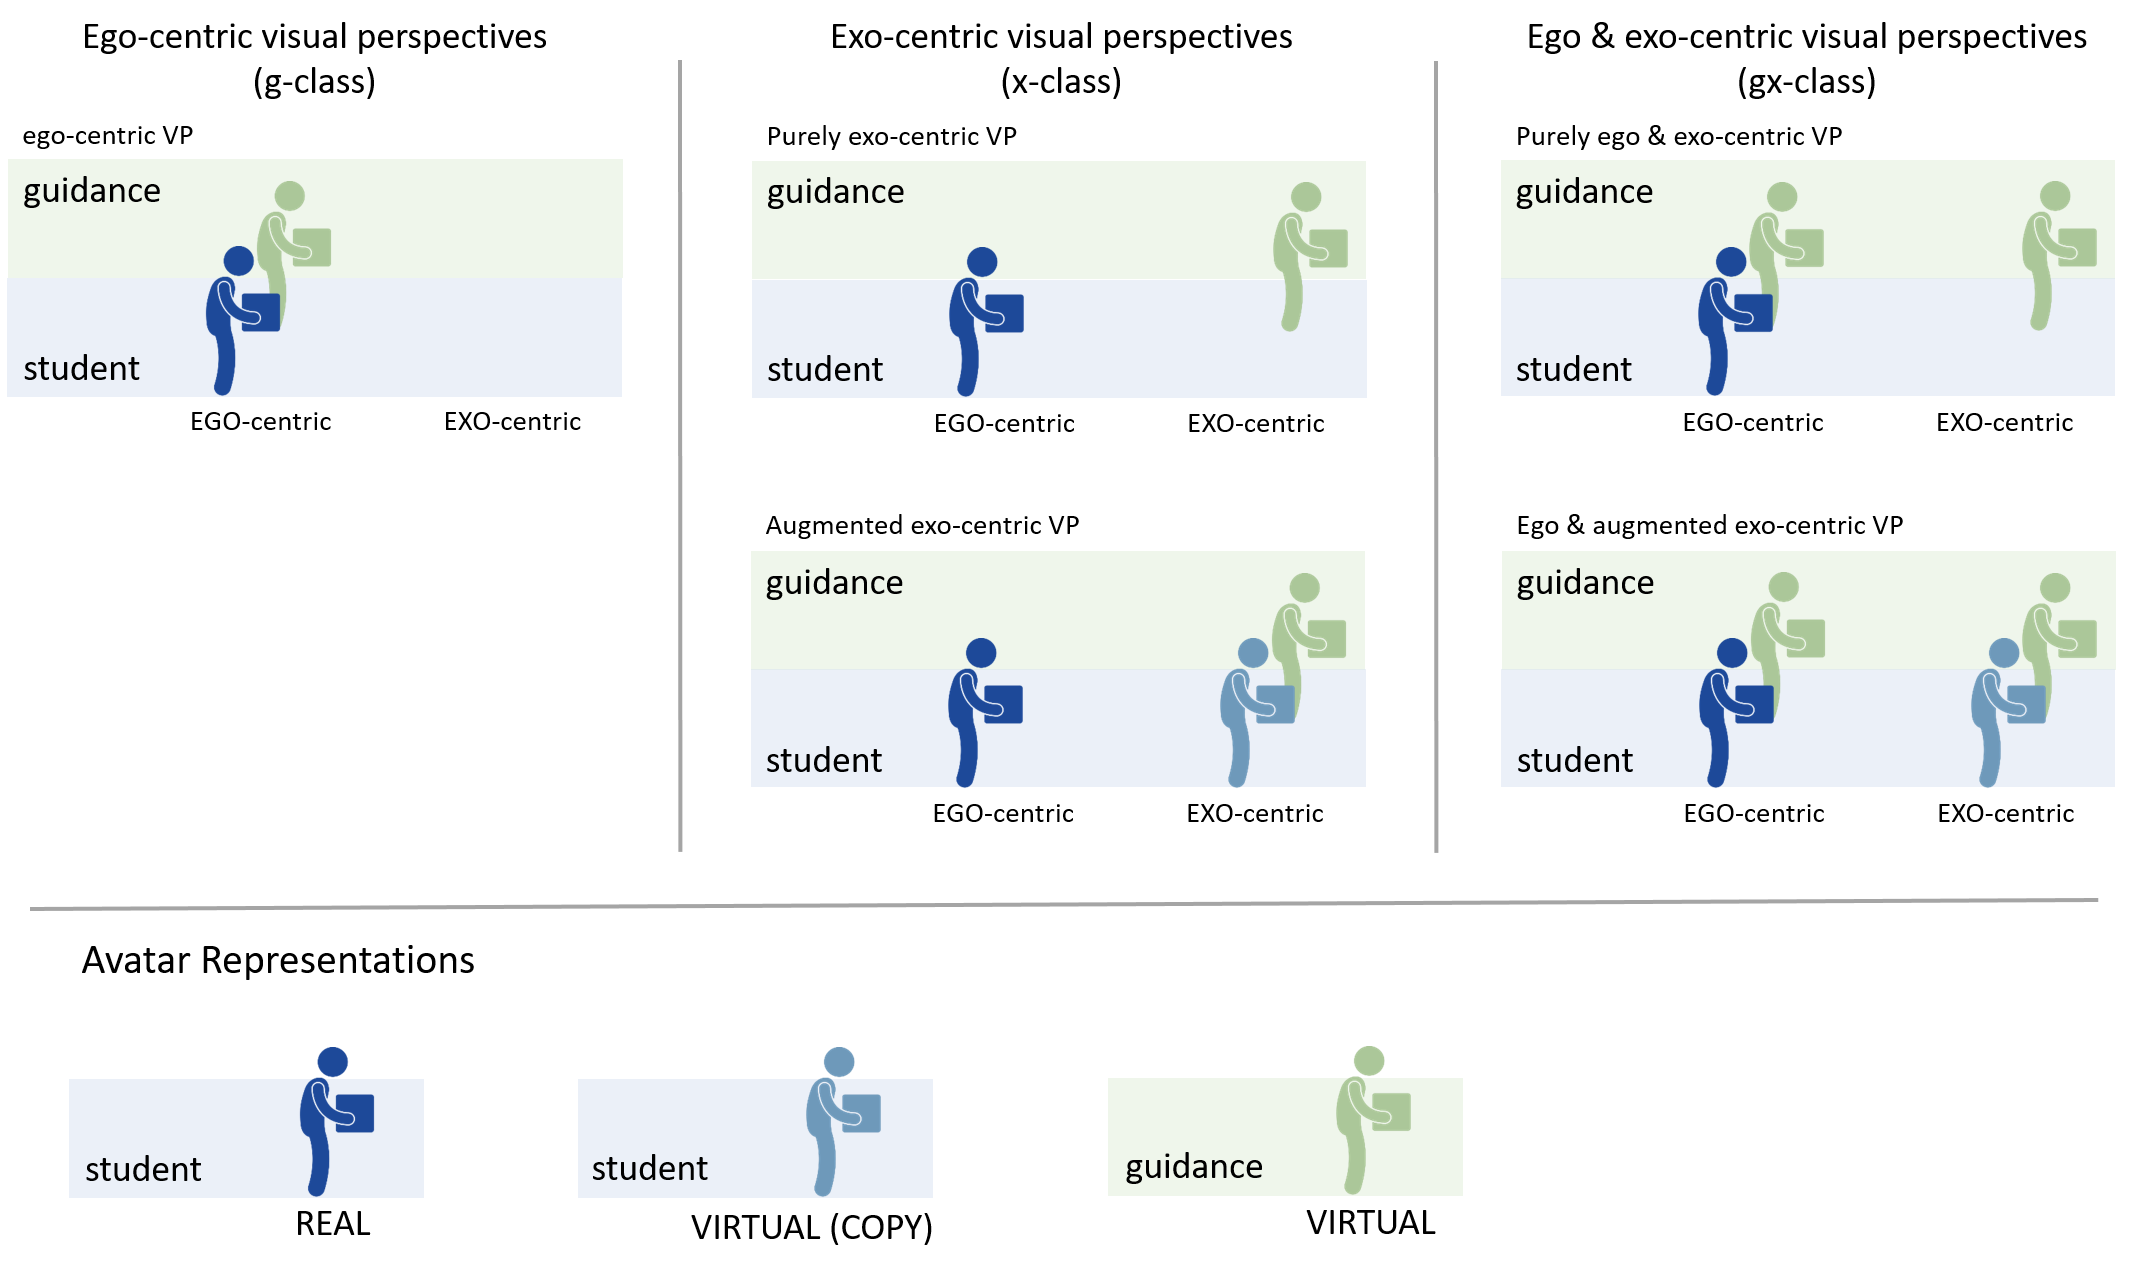
\includegraphics[width=\textwidth]{figures/perspectives_new.png}
	\caption[Visual perspectives on vitual guidance visualisations]{Visual perspectives on  virtual guidance visualisations, clustered by their corresponding class. Icon: created by Ghan Khoon Lay from Noun Project, \href{https://thenounproject.com/}{https://thenounproject.com/}, accessed: 19.06.2020}
	\label{fig:perspectives}
\end{figure}

\section{Handling Physical Load}
\label{section:handlingphysicalload}
Handling physical load is part of the more general topic Manual Material Handling (MMH). MMH is composed of five elemental tasks: lift, lower, push, pull and hold~\cite{mmh}. Additionally, there are non-elemental tasks like turning and sliding (ibid.). This master's thesis will use a experiment task that include the handling of physical load. Evidently, the task should consist of these elemental tasks. A task that consists of elemental tasks can be generalised to other tasks to a certain extend. To gain a stronger data basis, multiple elemental tasks can be chained together and repeated, to form a so-called Unit-Combined-MMH (ibid.). In chapter~\ref{sec:taskDesign} is described how the elemental tasks become subtasks of the experiment task.

\section{Injury Risk Metrics}
\label{section:rm}
Muckell et al.~\cite{muckell} identified four main features which are common in the bio-mechanical evaluation of different lifting and carrying techniques. Based on those four features, they defined four injury risk metrics to define low risk and high risk movements. The four risk metrics (RM) are described in the following. \textit{Support base} describes the distance between the feet. With a proper support base, an individual is more stable while performing a movement like lifting or lowering. \textit{Squat} describes the distance between pelvis and floor. "A proper \textit{squat} reduces injury risk, since the lifting force is applied using legs and not the back" (ibid.). \textit{Upright stance} is defined by the angle between the upright vector and the bend of the back of an individual. \textit{Spine twist} is the angle between the lines between the left and right shoudler and the left and right hip.

\section{Related Work: Motor Learning in Virtual Reality}
\label{section:related_work}
\begin{table}[H]
	\begin{tabularx}\textwidth{@{}XXXX@{}}
		\toprule
		g-class & x-class & g-class and x-class & gx-class \\ \midrule
		AR-Arm \cite{ararm} & MotionMA \cite{motionma} & OneBody \cite{onebody} & Tai Chi Trainer \cite{thaichichua} \\
		Just Follow Me \cite{justfollowme} & YouMove \cite{YouMove} & LightGuide \cite{lightguide} & SleeveAR \cite{sleevear} \\
		Ghostman \cite{ghostman} & VR Dance Trainer \cite{vrdancetrainer} & MR Dance Trainer \cite{mrdancetrainer} & \\
		Stylo Handifact \cite{stylo} & Physio@Home \cite{physioathome} & Throw Simulator \cite{freethrowsimulator} & \\
		GhostHands \cite{ghosthands} & OutsideMe \cite{outsideme} & Training Phys. Skill \cite{trainingphysicalskills} & \\
		& E-Learning MA \cite{elearningma} &  &  \\
		& My Tai Chi \cite{mythaichicoaches}  & &\\
		& Perform. Training \cite{performancetraining} & &\\
		& RT Gestrue Recognition \cite{rtgesturerecognistion} & &\\
		& KinoHaptics \cite{kinohaptics} & &\\
		& TIKL \cite{tikl} & &\\ \bottomrule
	\end{tabularx}
	\caption[Related work clustered by the visual perspectives.]{Overview of related work clustered by visual perspectives.}
	\label{tab:rw_overview}
\end{table}

Training movements in Virtual Reality were investigated previously in several works. An overview differentiated by the VP the reasearchers used to train movements is provided in~\ref{tab:rw_overview}. AR-Arm~\cite{ararm}, Just Follow Me~\cite{justfollowme}, Ghostman~\cite{ghostman}, Stylo and Handifact~\cite{stylo} and GhostHands~\cite{ghosthands} used the ego-centric VP. MotionMA~\cite{motionma}, YouMove~\cite{YouMove}, VR Dance Trainer~\cite{vrdancetrainer}, Physio@Home~\cite{physioathome}, OutsideMe~\cite{outsideme}, E-learning Martial Arts~\cite{elearningma}, My Tai-Chi coaches~\cite{mythaichicoaches}, Performance Training~\cite{performancetraining}, Real Time Gesture Recognition~\cite{rtgesturerecognistion}, KinoHaptics~\cite{kinohaptics} and TIKL~\cite{tikl} used a VP from the g-class. There are also works that used to train movements in g-class and x-class, like OneBody~\cite{onebody}, LightGuide~\cite{lightguide}, Mixed Reality Dance Trainer~\cite{mrdancetrainer}, Free Throw Simulator~\cite{freethrowsimulator} and Training Physical Skills~\cite{trainingphysicalskills}. It is little research done for movement training in the gx-class, for example Tai Chi Trainer~\cite{thaichichua} and SleeveAR~\cite{sleevear}.\\
The task which the refferred works use araise from the fields of dancing~\cite{YouMove,vrdancetrainer,outsideme,performancetraining,mrdancetrainer}, sports~\cite{freethrowsimulator,trainingphysicalskills}, rehabilitation~\cite{motionma,physioathome,kinohaptics,sleevear,veimprovesml}, arts~\cite{ararm,justfollowme,stylo,elearningma,mythaichicoaches,rtgesturerecognistion,onebody,thaichichua} and others~\cite{tikl,lightguide}. None of them include the ergonomic handling of a physical load, but sometimes include physical artefacts like a ball (e.g. Free Throw Simulator~\cite{}) or chop sticks (Ghostman~\cite{ghostman}). Also none include locomotional movements.\\
The body parts that are included in the above mentioned task vary, too. For example, \cite{YouMove, thaichichua,onebody,vrdancetrainer} full body movements are taken into consideration, while \cite{ararm,sleevear,ghosthands} uses arm movements.\\
The guidance visualisations which are used to train movements are stick figures~\cite{onebody,YouMove,vrdancetrainer,performancetraining}, wireframes\cite{thaichichua,mrdancetrainer}, human-shaped avatars\cite{thaichichua,vrdancetrainer,trainingphysicalskills,mythaichicoaches} and indicators~\cite{ararm,physioathome,sleevear,ghostman}.\\
To determine to what extend the movements of the learner matcher the GV, different measures are applied. Most common are performance measures based on the accuracy of the performend movements (e.g.~\cite{YouMove,thaichichua,vrdancetrainer,onebody,lightguide,physioathome}) and the time related measurements like the task completion time (e.g.~\cite{lightguide,onebody}).\\
How the perspective influences the learners performance is sparsely investigated. Recently, in December 2020, Yu et al.~\cite{perspectivematters} conducted three independent studies to close this gap. In the first study, Yu et al. compared the ego-centric visual perspective and a 2D-mirror for single arm movements. In the second study, they compared the ego-centric and exo-centric visual perspective for Yoga. In the third study, they compared the ego-centric visual perspective with a 3D-mirror for arm movements. Yu et al. conclude their findings in a design guideline for systems training motor learning in Virtual Reality: use the ego-centric visual perspective if the type of motion allows, consider alternatives for other types of motions, ibidem. In all three studies, the ego-centric visual perspective outperformed the other perspectives if the movement was completely visible from the ego-centric visual perspective. \cite{onebody,lightguide} compared their ego-centric VP with their exo-centric VP and for the task they used, the ego-centric VP outperformed the exo-centric VP. \cite{YouMove,vrdancetrainer} compared the movment learning in VR with traditional video based movement learning. In both cases, VR movement learning outperformed video movement learning.\\

\subsection{Research Contribution Statement}
\label{sec:delimination_contribution}
As depicted in the last section, motor learning in the gx-class VPs is rarely investigated, especially for full body movements. Furthermore, motor learning that includes the handling of a physical load in VR in different VPs was not part of investigations. Additionally, previous works used stationary task in the ego-centric VP. Moreover, how the visual perspectives influence the learners visual focus is unexplored.\\
The proposed experiment in this master's thesis will provide an empirical contribution by increasing the empicial evidence of how the VP on GVs influences motor learning by guiding full body movements in three VP: ego-centric, exo-centric and the pure combination of them. Furthermore, empirical evidence is generated for motor learning including the handling of a physical load and the learners visual focus. An artifact contribution is provided by presenting a method for guiding locomotion movements in the ego-centric VP. \\

The generated data of the proposed experiment will help designers of VR motor learning systems to choose a reasonable perspective for their project.


%The preceding seminar thesis provided an overview over 23 (compare table~\ref{tab:rw_overview}) of these works and evaluated six of them in detail: Tai Chi Trainer by Chua et al.~\cite{thaichichua}, YouMove by Anderson et al.~\cite{YouMove}, VR Dance Trainer by Chan et al.~\cite{vrdancetrainer}, OneBody by Hoang et al.~\cite{onebody}, LightGuide by Sodhi et al.~\cite{lightguide} and Pyhsio@Home by Tang et al.~\cite{physioathome}. Special attention was paid to the VP, task, GV and their independent and dependent variables they used in their investigations. Finally, the results of these works were concluded. An overview is depicted in table~\ref{tab:rw_overview_detail}.

%These works inform this work in various aspects. Chua et al. used the ego \& augmented exo-centric VP, Hoang et al. and Sodhi et al. the ego-centric visual perspective. These visual perspectives proved to be suited for the evaluation of Motor Learning in VR and is adopted for the proposed study design, compare section~\ref{section:visual_perspectives}. Furthermore, Chan et al. and Chua et al. used high realistic avatars as guidance visualisation, which are used in the proposed study design, compare seminar thesis chapter 3.3. Additionally, recent research indicates that high realism avatars outperform abstract avatars~\cite{max,perspectivematters}. All authors used a performance measure to evaluate the performed movements of the participants of their studies. Primarily the distance-based measures informed the measures used in the proposed study design\\%compare figure ??? yxc
%The above mentioned works do not use the relatively new technology of Vive Trackers in combination with Inverse Kinematics (IK, see project report chapter 2.1 and 2.2). Sra et al.~\cite{samesetup} used this technology in 2018 for their system Your Place and Mine to render human-shaped avatars.\\
%The results of related work yielded no clear conclusion about the influence of the perspectives on motor learning. Chua et al. found no difference in the performance between the visual perspectives, Anderson et al. and Chan et al. found out that their exo-centric visual perspectives in Virtual Reality outperform traditional video guidance. Hoang et al. and Sodhi et al. conclude that the ego-centric perspective outperforms the exo-centric visual perspective. Nevertheless, an investigation of how the visual perspective influences motor learning was not investigated.  This work, in contrast, focuses on full-body movements that include the handling of physical load. Furthermore, this work provides a third visual perspective, where the ego-centric and exo-centric visual perspective is combined.

%VR already proved to be a suitable environment for Motor Learning for tasks like dancing~\cite{YouMove,vrdancetrainer,outsideme,performancetraining,mrdancetrainer}, sports~\cite{freethrowsimulator,trainingphysicalskills}, Rehabilitation~\cite{motionma,physioathome,kinohaptics,sleevear,veimprovesml}, arts~\cite{ararm,justfollowme,stylo,elearningma,mythaichicoaches,rtgesturerecognistion,onebody,thaichichua} and others~\cite{tikl,lightguide}.
 



%\todo{new papers occured, read them, then write this statement. notes:}
%what is done:  v
%comparing ego-centric with exo-centric video.
%comparing ego-centric with exo-centric and the combination, but yielded to no result, because old paper and old pc
%comparing with mirrors,
%comparing isolated body parts
%everyone made his live easy by just looking at stationary movements, mostly containing only some body parts.
%new: nobody did fullbody movements with locomotion. ego-centric locomotion motion guidance is completely new. 
%related work only investigated on stationary movements. but motor learning is not stationary. body parts is also not stationary.
%real-world relation poor because of arts dance or abstract. my work is the first one haveing really a task that is reasonable!\\
%Previous work investigated the differences between the perspectives, but:
%To my knowledge, there is no investigation on full body movements that include locomotion. Furthermore, there are on investigations that include the handling of physical load.
%Perivous works compared ego-centric Motor Learning with video learning\cite{YouMove,vrdancetrainer}, augemnted mirrors\cite{perspectivematters,onebody}.
%The conduction of the proposed study will produce data that serves as a reasonable basis for designers of VR Motor Learning systems choosing a suitable perspectives. This is achieved by an Empirical Research Contribution. The empirical data is gathered by a comparative study between the ego-centric visual perspective, the exo-centric visual perspective and the combination. As novelty, the task includes handling of physical load which consists of the elemental tasks of manual material handling. This allows an evaluation of the elemental tasks per visual perspective and can give insights which perspective is suited for specific tasks.\\
%Additionaly, an artifact contribution is provided by the ego-centric guidance of locomotion movements.

%direct comparison not even in tai chi chua

%\chapter{Conceptual Delimitation and Contribution Statement}
abgrenzung zu related work und klares contribution statement\\
contribution type
\chapter{Experiment Design and System Implementation}
\label{chapter:studysetting_conduction}
\section{Experiment Design}
\label{section:study}

\subsection{Independet Variables: Visual Perspectives}
The last chapter pointed out five possible visual perspectives in a scenario with one teacher and one student, compare figure~\ref{fig:perspectives}. All visual perspectives are worth investigating, and a comparative study with all five visual perspectives is desirable. Though, to reduce complexity and the number of participants\footnote{Due to COVID-19 pandemic}, this work will focus on three visual perspectives.\\
Figure~\ref{fig:perspectives} shows three main classes of visual perspectives: ego-centric, exo-centric and perspectives which contain both. To answer the research question, it is indispensably to examine at least one of each class. The ego-centric VP is unique and though chosen by default. The exo-centric VP can be realised as purely exo-centric or augmented exo-centric. The combination of ego-centric and exo-centric can be realised as ego \& exo-centric or ego \& augmented exo-centric. However, before the exo-centric VP and the combination can be chosen, a closer look at the mechanics that makes Motor Learning in VR possible is necessary.

\subsubsection{Excursion: Mechanics for Motor Learning in Virtual Reality}
For teaching movements in Virtual Reality in the exo-centric VP, the following issue arises: the GV can move out of the learner's field of view by the movement itself. Szenario: the learner and the GV stand side-by-side. The learner sees the GV to the left. The GV now indicates a movement to turn by 90 degrees to the right. As soon as the learner follows this movement, the GV will be located behind the learner after the movement ended. The learner cannot see a GV standing behind the learner.\\
This issue is solved in existing work with either the restriction of movements~\cite{freethrowsimulator,elearningma} or multiple representations of the GV around the learner~\cite{thaichichua,mythaichicoaches}. The restriction of movements has a strong influence on the task design and is therefore not desirable for the study proposed in this thesis. Consequentially, for exo-centric visual perspectives, multiple representations for the GVs on strategic positions around the learner are necessary.\\
In the ego-centric visual perspective, another issue arises during the teaching of locomotion movements. To understand this issue, two aspects have to be clear before. (1) The nature of an ego-centric GV is to be located inside the learner at any time. (2) A GV indicates movements by moving itself. If the GV is about to indicate a movement away from the learner, the GV is moving out of the student's body. However, a GV that is outside of the learner's body is no longer ego-centric.\\
A possible solution is given by the centricity continuum by Wang and Milgram~\ref{fig:ego-exo-continuum}. Following the centricity continuum's nature, the tethering distance can be increased by a small amount, and the visual perspective can still be classified as ego-centric. But now arises the question of how far the tethering distance can be increased, with which the perspective still feels ego-centric, but the indication of the movement is considerable. For simplicity, this distance is further called ego-centric tethering distance (ETD). To determine a reasonable ETD, a formative study was conducted. During this study, one\footnote{A larger study was not possible because of the COVID-19 pandemic} non biased\footnote{The person had no prior knowledge about the system or motor learning.} person was asked to follow movements in the ego-centric visual perspective. The first movement was conducted with an ETD of 5cm. For the following movements, the ETD was increased by 5cm each. The subjective assessment of the participant and my observations yielded best for an ETD between 15cm and 30cm. These two values are further called:
\begin{itemize}
	\item[] $ETD_{min}=15cm$
	\item[] $ETD_{max}=30cm$
\end{itemize}
Based on $ETD_{min}$ and $ETD_{max}$ the speed mechanic is developed. The speed mechanic controls the speed of the playback of the GV. At $ETD_{min}$ and below, the animation plays at normal speed. At $ETD_{max}$ the GV stops. Between $ETD_{min}$ and $ETD_{max}$ the animation speed of the GV is linearly interpolated, compare figure~\ref{fig:speed_mechanic}.
\begin{figure}[htb]
	\centering
	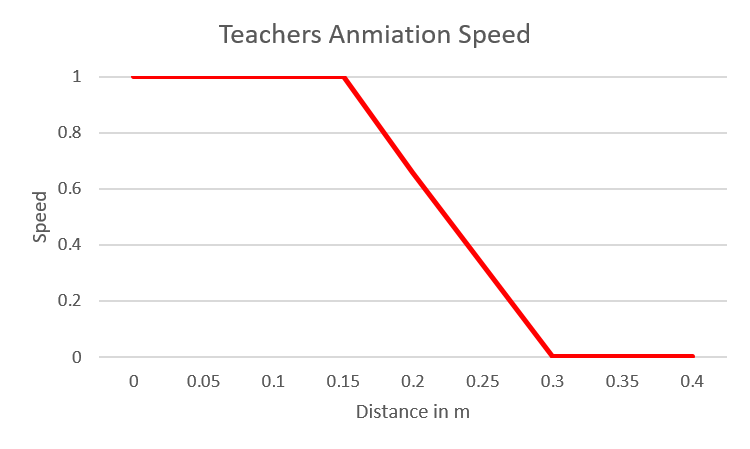
\includegraphics[width=\textwidth]{figures/speed_mechanic_chart.png}
	\caption[speed mechanic chart]{speed mechanic chart}
	\label{fig:speed_mechanic}
\end{figure}
The speed-mechanic was evaluated by one person\footnote{Different person than the first one. This person had no prior knowledge about the system nor Motor Learning. A Larger evaluation was not possible because of the COVID-19 pandemic.}. The participant followed the GV in the ego-centric visual perspective. Observations showed that the participant could follow the movement at ease. The opinion of the participant about the speed mechanic was very positive.\\
With this short excursion, a reasonable decision for the exo-centric VP and the combination can be chosen.\\

In the ego-centric visual perspective, the learner sees the GV inside the own body. Here, the learner can see the relation of the own body to the GV directly. In the pure exo-centric visual perspective, this relation cannot be seen. Thereby, the position of the learner in relation to the GV must be guessed. That, in turn, makes the application of the speed-mechanic - which is necessary for ego-centric guidance - not possible. A mechanic that is used in all conditions but one could lead to biased data, compare table~\ref{tab:mechanics}.
\begin{table}[htb]
	\centering
	
\includegraphics[width=\textwidth]{figures/mechanics_comparison.png}
	\caption[Mechanics for Motor Learing in Virtual Reality]{Mechanics speed and multiple representations and in which VP they are applied.}
	\label{tab:mechanics}
\end{table}
The mechanic of multiple representations does not influence the study's validity because the mechanic would solve an issue that does not exist in the ego-centric perspectives. Furthermore, any VP  with more than one representation is an exo-centric VP.\\
In the augmented exo-centric VP, a virtual copy of the learner is located inside the exo-centric GV. The copy lets the learner see the relation of the own body to the GV. Furthermore, augmenting the exo-centric GV with the learner is widely used and evaluated in related work~\cite{YouMove,thaichichua}. Consequently, the augmented exo-centric VP will serve as the exo-centric VP.\\
With the ego-centric and exo-centric VP set, the combination can be chosen. In the ego-centric VP, the learner has a direct comparison of the own posture to the GV posture in the ego-centric VP. In the augmented exo-centric VP, the learner has a direct comparison of the own posture and the GV posture in the exo-centric VP. For a direct comparison of the ego-centric VP AND the exo-centric VP, the ego \& augmented exo-centric VP is chosen as the combination. The ego \& augmented exo-centric VP is the true combination of ego-centric and augmented exo-centric.\\
For simplification, the augmented exo-centric VP will be further called exo-centric VP, and the ego \& augmented exo-centric will be further called ego \& exo-centric VP.\\
The ego-centric VP, exo-centric VP and the ego \& exo-centric VP are the independent variables of the study and form the three study conditions EGO, EXO, EGO \& EXO.

\subsection{Task Design}
Hornb\ae{}k~\cite{hornbaek} identified three main types of tasks in HCI studies: representative tasks, simple tasks and tasks that use task-specific hypothesis. RQ1 states that the main investigation field is Motor Learning. Motor Learning is strongly related to real-world movements. Evidently, the study task is a representative task.\\
Real-world tasks that include the handling of physical load can found in a wide range of activities. For example, a storekeepers job is to clear a palette of cardboard boxes. This task includes unloading the palette, scale the boxes, measure the dimensions of the boxes and finally store them in a rack. Another example is the work at a grinding machine. The worker takes a slug from a shelf and works on it until the slug becomes a workpiece. After that, the workpiece is carried to a measurement instrument to be verified. There are plenty of other examples, but these two already clarify that tasks which include the handling of physical load consist out of the elemental tasks for manual material handling: lift, lower, push, pull, hold.\\
The study task's idea is to chain these elemental tasks together to a Unit-Combined-MMH task that representatively stand for a wide range of tasks that includes the handling of physical load. To achieve this, several aspects have to be taken into consideration: (a) the artefacts with which the learner will interact, (b) a reasonable task decomposition that allows the investigation of sub-tasks. Furthermore, the study needs a (c) structure. (c) will reveal the necessity of three tasks. These tasks have to be equally (d) complex. This section will subsequently discuss (a-d) and propose the task for the study.

\subsubsection{(a) Artifacts}
A task that includes the handling of physical load obviously needs a physical load. In real-world tasks, the physical load can be everything a human can handle. The physical load for this task should fulfil the following criteria. First, the load should have a significant weight, that it is perceived as a load, but at the same time, any healthy person with no previous illnesses can handle it without getting injured. Secondly, the physical load should give enough freedom for interactions. A simple box fulfils the criteria and has a relation to physical loads of real-world tasks like the handling of parcels. With a physical load, the elemental tasks of lift and lower can be realised by lifting and lowering the box from and to the floor.\\
Push and pull can be realised by pushing and pulling the box on the floor, but it can feel cumbersome. Moreover, in real-world task pushing and pulling a box is made possible in a more ergonomic height if possible, not least for security reasons. To support push and pull, a table is introduced. This table stands representatively, for example, the grinding machine or a parcel sorting table.\\
Finally, the transitions between the elemental tasks have to be supported to increase the real-world reference. This is achieved by providing a waypoint. The waypoint is a plate on the floor and helps to bring sense in movements. This plate representatively stands, for example, for a scale or second machine. Walking to a scale or lower a box to the scale on the floor increases the real-world reference more than just an empty place in the room.

\subsubsection{(b) Sub-tasks}
\label{sec:subTasks}
The goal is to create a Unit-Combined-MMH task with the elemental tasks push, pull, lift, lower and hold. The process of designing the task is complex and took place iteratively.\\
The first approach was a task with four occurrences of every elemental task. For lifting the box from the scale and carry the box to the table, obviously, a new task type had to be introduced: carry. Because carry is not an elemental task and for simplicity, elemental tasks and newly introduced task types are referred to as sub-tasks. This first approach of designing a task revealed an issue: chaining a given amount of sub-tasks together so that the task is still conductible is hard to achieve. To overcome the inflexibility in task design, a new sub-tasks is introduced: walk. Walk means locomotion without the box in hand. With walk, the box can be pushed from one side of the table and then be pushed from the other side of the table, which achieves flexibility in task design. Otherwise, on push will always follow pull.\\
The following approach was a task that consists out of the sub-tasks push, pull, lift, lower, carry, walk and hold. Each sub-task appeared four times. The task was evaluated with one\footnote{larger studies covid} person. This person had to follow the instructions in the ego-centric VP and exo-centric VP. During the task's conduction, the person started to look around and correct the own position during the sub-task hold. An interview afterwards showed that the person thought the GV stopped because his position was too far away from the GV. It became clear that the speed-mechanic and the sub-task are not compatible. It is indistinguishable for the study participant if he/she is too far away from the GV or if it is the sub-task hold. Because of this indistinguishableness, the sub-task hold is excluded from the task. However, hold is still part of the whole tasks: between the transitions of the tasks (for example, between lift ends and lower starts) is a slight pause which is equivalent to hold, but this sequence is to short to log. Furthermore, hold is part of the sub-task carry, where the box is held in front of the body. However, hold is not a stand-alone sub-task and though can not be evaluated isolated.\\
A new task was designed with the sub-tasks push, pull, lift, lower, carry and walk. During the design, special attention was paid to the magnitude of the movements. For example, every push should be equally far. Lift and lower from and to the scale and lift and lower from and to the table are very diffrent in the magnitude. This resulted in two new sub-tasks: pick and place. Pick means to pick up the box from the table, place means to place the box on the table, while lift and lower the target remained the scale on the floor.\\
The next stage of the task consists out of the sub-tasks push, pull, lift, lower, carry, walk, pick and place. The task was inspected by a professional physiologist. The physiologist was asked to describe the sub-tasks in detail and perform every sub-task ergonomically. The professional's description of the sub-tasks are listed in table~\ref{tab:sub-tasks}. From the performance of the professional physiologist and the description of the sub-tasks could be derived several insights. The sub-tasks push and pull are very similar in their conduction. The same applies to the pairs lift and lower as well as pick and place. This meant for the evaluation that the variations of movements are nearly halved, and the possibility of making mistakes is reduced. Example: for push and pull, one foot has to be placed to the back while the other foot remains under the hip. The hands do the same for every push and pull. If the participant does perform the sub-task intrinsically correct without the perception of the GV, the study will not measure the influence of the perspective. To increase the number of sources of error, two new sub-tasks are introduced: turn and fold. Turn means to turn the box by 90 degrees on the table. Fold means to tilt the box from one side to another. The difference in hand movement to push and pull is obvious. The difference for the feet results from the fact that during turn and fold, the box's weight remains on the table. The force to apply on the box is significantly lower than during push and pull. This results in a different feet placement, which is hip wide under the hip.\\
With the introduction of turn and fold, all sub-tasks are introduced. A new task was created with all ten sub-tasks. To assess all sub-tasks multiple times, they appear four times per task. The pair lift and lower and the only in magnitude different pair place and pick relate to each other. To be presented equally in the task among the other sub-tasks, they should also only be present four times. Because lift and lower are measured with the RM (6.2) (see next section), lift and lower was decided to appear three times each, and pick and place one time each. Unfortunately, only one time each pick and place means that all sub-tasks that do not happen at the table had to be conducted in sequence. To regain flexibility in the task, it was decided that pick and place will occur two times each. This results in 34 sub-tasks per task. Table~\ref{tab:sub-tasks} provides an overview of the sub-tasks and their corresponding description, as well as the occurrences per task.

\begin{table}[H]
	\centering
	
\includegraphics[width=\textwidth]{figures/sub_tasks_definition.png}
	\caption[Description of sub-tasks]{Sub-tasks that appear in every task.}
	\label{tab:sub-tasks}
\end{table}

\subsubsection{(c) Study Structure}
\label{sec:studyStructure}
In the study, three conditions are compared: EGO, EXO and EGO \& EXO. The main question of this section is how to assign the participant to the independent variables. The key distinction is between within-subject design and between-subject design~\cite{hornbaek}. In the within-subject design, the participant would experience all VPs. In the between-subject design, the participants would experience only one VP. Within-subject designs typically can detect the differences between the conditions more precisely (ibid.). Furthermore, within-subject designs need less participants~\footnote{The COVID-19 pandemic makes it hard to find enough participants.} than between-subject designs (ibid.). For these reasons, the study is conducted in a within-subject design.
The within-subject design also has a drawback: the participants gain experience about the task and the conditions during the study. This means that one condition is influenced by another condition, which the participant already experienced. Furthermore, there is an asymmetrical carry-over effect between the conditions: EGO \& EXO contains condition EGO and EXO and thereby influences EGO and EXO more than EGO and EXO influences EGO \& EXO. To reduce the task related learning effect, three tasks with nearly equal complexity are created. With this, a participant will face for every condition a different task. The tasks are still similar, and the learning effect persists. A reduction of the influence of the learning effect on the outcome can be countered out by counterbalancing the task. Like the task, the carry-over effect between the conditions can also be countered by counterbalancing the conditions. Hornb\ae{}k proposes, in this case, to cross the conditions with the task and use a Greco-Latin square. Three conditions and three tasks in Greco-Latin square results in blocks of nine participants. This block is depicted in figure~\ref{fig:study_session_plan}. The study should be conducted with at least four blocks (4x9=36 participants) \todo{warum?????}. The first session of every study is for acclimatisation and is excluded from evaluation.

\begin{figure}[htb]
	\centering
	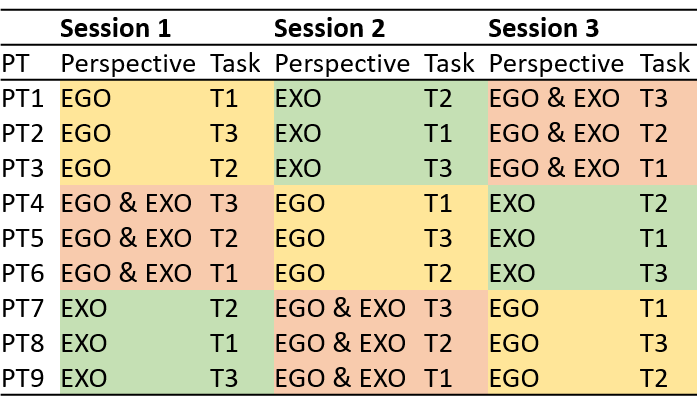
\includegraphics[width=0.5\textwidth]{figures/study_session_plan.png}
	\caption[Study structure]{Experiment structure: within-subject desing in a Greco-Latin square.}
	\label{fig:study_session_plan}
\end{figure}

\subsubsection{(d) Equal Task Complexity}
A study participant will face in every condition another task. For the study's validity, it is indispensable that these three tasks have nearly equal complexity. As described in (b), a task consists of 10 subtasks that occur a specific amount. The main idea to ensure a comparable complexity is to use the sub-tasks for all three tasks in an equal amount. This means the 34 sub-tasks of task one occur in task two and three but in a different order. Table~\ref{tab:tasks} lists all three tasks. For every task, the sub-task number ST1-ST34 is provided. Every sub-task number stands for a sub-task, which comes with a description and the sub-task ID. Reading the description from top to bottom are the instructions the learner receives from the GV during one condition. The mirror mentioned in the first line is another waypoint, which is necessary for technical reasons and is described in section~\ref{sec:selfperception}.

\begin{table}[H]
	\centering
	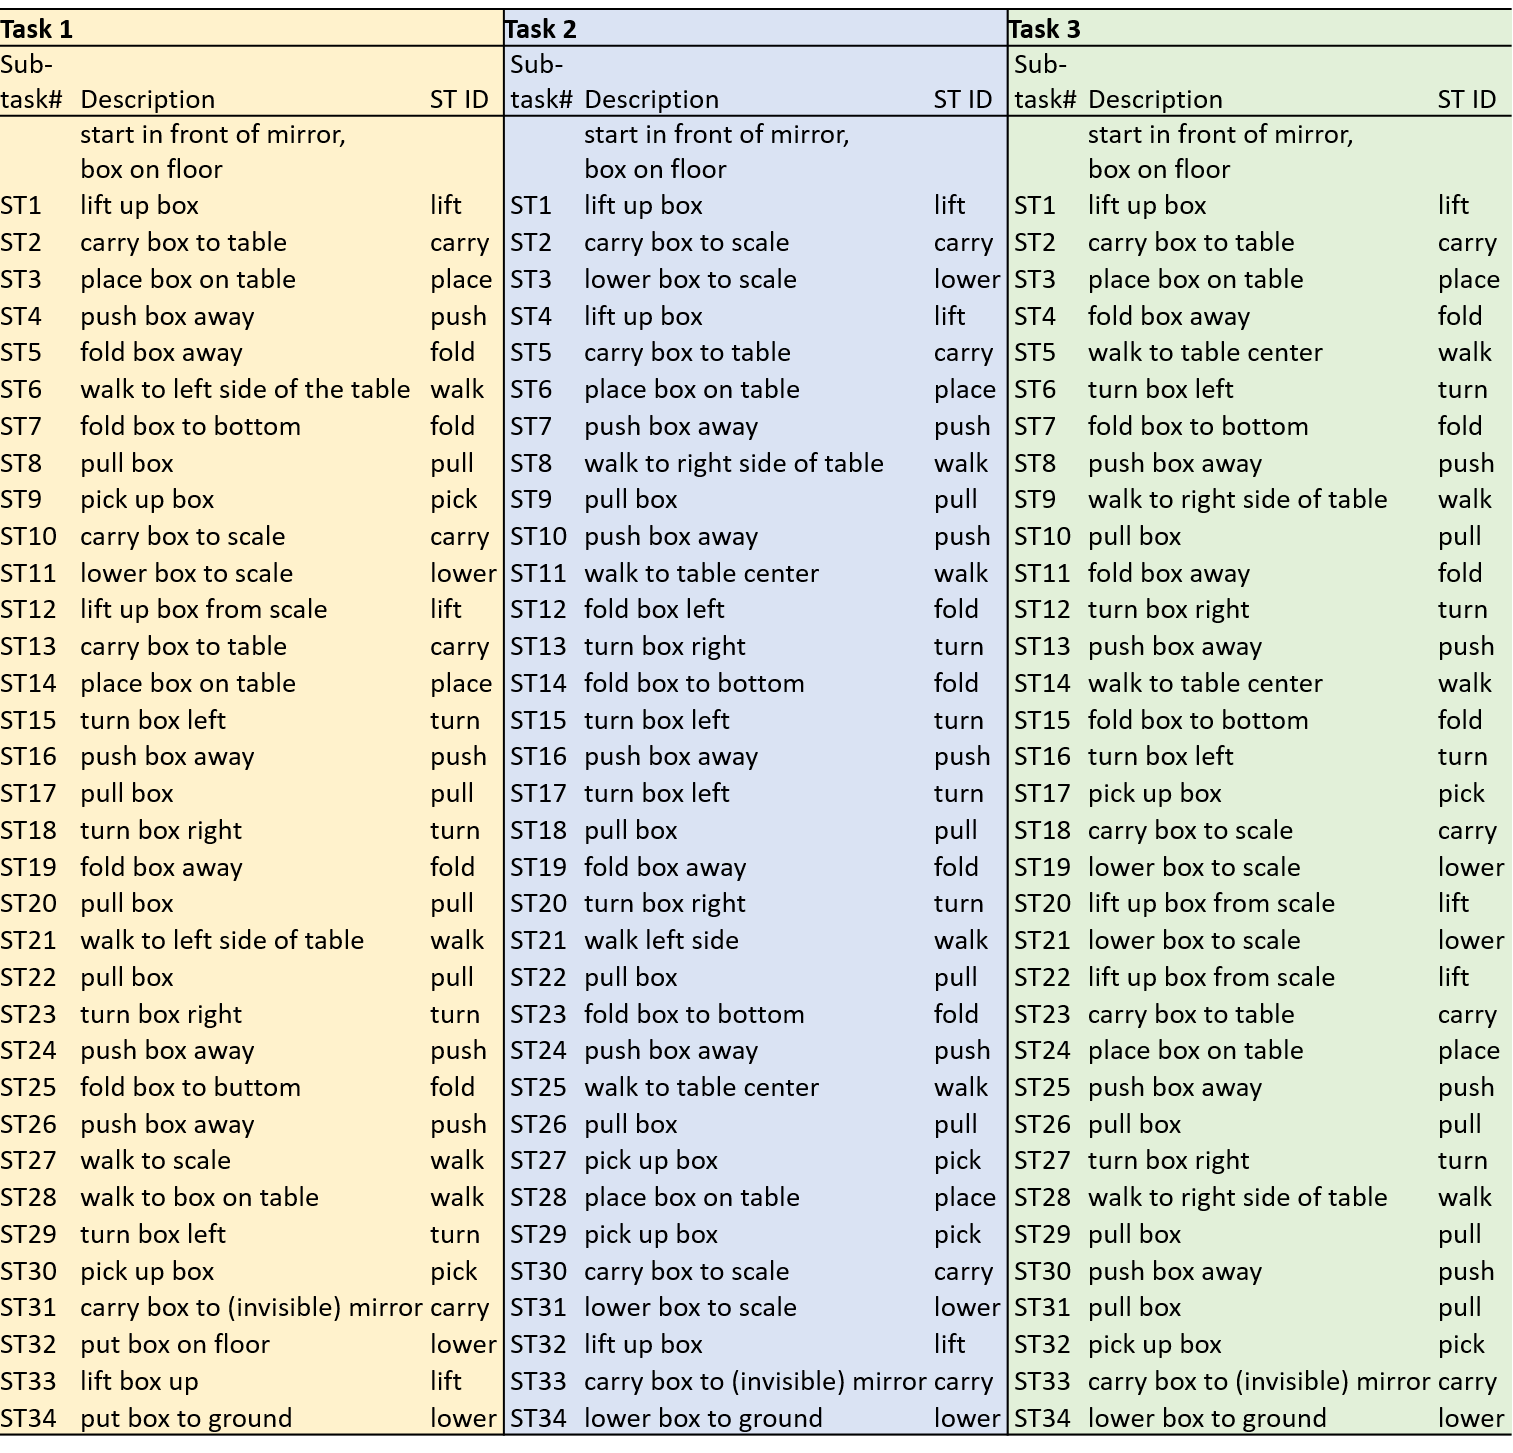
\includegraphics[width=\textwidth]{figures/tasks.png}
	\caption[Description of tasks]{tasks}
	\label{tab:tasks}
\end{table}

\subsection{Measures: dependent variables}
\label{sec:measures}
This works aim is to answer the main research question RQ1: How does the visual perspective on a virtual GV influence Motor Learning in Virtual Reality. To answer this research question, the proposed study has to generate data that can answer the sub-research questions RQ1.1-4. This section will provide the underlying paradigm to every sub-research question and explain which measures are necessary.\\

\textbf{RQ1.1} How does the visual perspective on a virtual guidance visualisation influence movements' accuracy?\\
\textbf{Paradigma:} The more exact the learner's movements matches the GV movements, the better the learner could follow the instruction of the GV. For RQ1.1.1, the limbs of the learner and the limbs of the GV are compared. For RQ1.1.2, the box' accuracy is compared. For RQ1.1.3, both are compared and additionally, the current sub-task is taken into consideration. The accuracy can indicate how the particular movement is suited for the VP.
\begin{itemize}
	\item[] \textbf{RQ1.1.1} How does the visual perspective on a virtual guidance visualisation influence movements' accuracy of the own body?\\
	\textbf{Measures}: (1) Euclidean distance between the learners and GVs hands, feet, head and hip in meters. (2) Angle between learners and GVs the hands, feet, head and hip in degrees.
	
	\item[] \textbf{RQ1.1.2} How does the visual perspective on a virtual guidance visualisation influence the accuracy of handling physical load?\\
	\textbf{Measures}: (3) Euclidean distance between the learners and GVs physical load. (4) Angle between the learners and GVs physical load in degrees.
	
	\item[] \textbf{RQ1.1.3}How does the visual perspective on a virtual guidance visualisation influence sub-tasks accuracy?\\
	\textbf{Measures}: (1-4), additionally matched to the sub-tasks that is currently performed (5).
\end{itemize}	
(1-4) gives insights to what extend the learner could follow the GV for the whole task. (5) can extract specific sub-tasks for which the learner could follow the GV to a certain extend. For example, in the ego-centric VP, the overall accuracy for a task is lower than in the other VPs, but the accuracy for the sub-tasks lift and lower is higher than in other VP. For this example, measure (5) can extract specific sub-tasks that are performed better or worse than in other VPs.\\

\textbf{RQ1.2} Does the visual perspective on a virtual guidance visualisation influence the transfer of ergonomic principles?\\
\textbf{Paradigma:} the more exact the learner's RM matches the GVs RM, the better the ergonomic principles could be transferred.\\
\textbf{Measures:} (6) Risk Measurements: (6.1) spine bend in degrees, (6.2) squat distance in meters, (6.3) good base in meters \todo{check names}, (6.4) box near body.\\
Muckell et al.~\cite{muckell} used four RM in their work to assess the performance of the conducted movements. Three of them are assessed in the proposed study, too.
\begin{itemize}
	\item[] (6.1) spine bend is defined by the difference in degrees between the straight upward vector and the back of the learner. For all sub-task, spine bend should be in a certain window. This window is calculated form the teacher, who recorded the movement. Spine bend indicates if the learner could percept the correct posture of his back.
	
	\item[] (6.2) squat distance is defined by the distance in meters between the feet. For the sub-tasks lift and lower, the squat distance should be in a specific window. This window is calculated form the teacher, who recorded the movement. For the other sub-tasks, squat distance is not applied because the knees do not bend in the other sub-tasks. Squat distance indicates if the learner could percept that he should bend his knees during lift and lower.
	
	\item[] (6.3) good base is defined by the distance in meters between the feet. For the sub-tasks push, pull, turn, fold, lift, lower, pick and place, the squat distance should be in a specific window. This window is calculated form the teacher, who recorded the movement. Good base indicates if the learner could percept the correct posture of the feet.
	Muckell et al.\cite{muckell} additionally use the RM spine twist in their work. This RM cannot be applied for this study because of the multiple perspective mechanic. The learner has multiple GV around and is free of choice which one to look at. The turn of the head implies spine twist. Though, spine twist has a low validity and reliability.
	
	\item[] (6.4) box near body. For the study task design, a professional physiologist was consulted (compare \todo{section}). During the interview, all movements were described in detail, compare \todo{figure}. During the sub-task carry, the box should be as near as possible to the body, while the elbows should have a bend angle of 90 degrees. Unfortunately, the bend angle could not be determined during a study for technical reasons, see chapter \todo{implementation}. Fortunately, the distance between the box and the body can be determined. Box near body is defined as the distance in meters between the box and the body of the learner. For the sub-task carry, box-near-body should be in a certain window. The window is calculated from the teacher who recorded the movement.
\end{itemize}

RM (6.1-4) are different from accuracy measurements (1-5) because they are independent of the learner's position and the GV. For example, in the exo-centric VP, a learner cannot percept the correct position where he/she should stand. The learner thereby stands 15cm away from the position he/she should stand. The overall accuracy is thereby lower. But the learner could percept the positioning of his/her feet correctly. In this case, the RM (6.3) are fulfiled while the accuracy is biased.\\

\textbf{RQ1.3} How does the visual perspective on a virtual guidance visualisation influence the learner's visual focus?\\
Measures: (7) looking at\\
Paradigma: the learner's visual focus is on the object the learner is looking at.\\
The learner interacts with a box and has multiple GVs around and inside the learner. Looking at can give insights on which GV the learner is focusing, the frequency of focus changes and the role of the physical load.

\textbf{RQ1.4} What is the subjective personal preference of the learner for the visual perspectives?\\
Measures: (8) qualitative data; Likert scales, semi-structured interview, digging into occurrences.\\
The qualitative data serves not only to investigate the learner's personal preference but also to serve as triangulation method (1-7).\\

The last measure is the (9) task completion time measured in milliseconds. The speed-mechanic regulates the speed of the animation of the GV. The further the learner is located to the GV, the slower the GV animation speed until it stops entirely at $EDT_{max}$. The task completion time can give insights into what extent the learner could perceive the desired position of his/her body in relation to the GV. This measure relates to (1) and can be used for triangulation.
Additionally, it is to expect that the TCT is decreasing from condition to condition because the participant acclimated. By that, TCT could give insights into the learning effect between the conditions. Finally, the study is recorded by video. If during the evaluation arises questions about a specific topic, the recordings can be consulted.

\section{\exgo - Design and Implementation}
\label{section:system}
The last section describes an experiment to investigate the influence of the visual perspective on Motor Learning in Virtual Reality. For the conduction of this study, a system is necessary. This system is called \exgo. This section elucidates the development of \exgo. The starting point is the creation of a self-perception of the learner. Section~\ref{sec:selfperception} describes how the learner gets a digital body in Virtual Reality. After that, in section~\ref{sec:perspectives}, the VPs have to be implemented, which in the study serve as the conditions. Section~\ref{sec:recording} deals with the recording of the movements of task 1-3. Section~\ref{sec:limitations}

\subsection{Self-Perception}
\label{sec:selfperception}
There are various options of devices to dive into Virtual Reality. In the preceding project report, several devices have been evaluated, and the decision was made for the Valve Index\footnote{\todo{todo}}, because of its refresh rate, screen solution and the possibility to wear glasses underneath the head-mounted display (HMD). To determine, the position and orientation of the HMD, the so-called Lighthouse\footnote{lighthouse} is utilised. A Lighthouse is tracking volume spanned by at least two Base-Stations\footnote{base stations} at the opposite corners of the room. To improve the tracking and for the avoidance of untracked areas, e.g. under the table, \exgo uses four base-stations, one for each corner fo the room, to span the Lighthouse.\\

Till now, the learner can move in an empty virtual world, seeing nothing. The next step is to replace the empty virtual world with a meaningful environment. For this, the Game Engine Unity 3D\footnote{Unity} is used. In Unity, a basic room was created. Four light yellow walls, a parquet floor and unidirectional lighting. The parquet floor serves a purpose: it has a structure with frequent straight lines, making it later easier to align the artefacts like table and scale. The room is kept simple not to distract the participant of the study.\\

The next step is to add the learner's body to this room. To achieve this, the body of the learner needs to be tracked. In the preceding project report, multiple full-body tracking systems were compared. The decision was made for Vive Trackers\footnote{Vive trackers}, because cease of coordinate system matching, the lower latency and less work-intensive calibration process. The learner wears six Vive Tracker in total. Five of them plus the HMD are necessary for the full-body tracking of the learner. The remainder is necessary for RM (6.1), which is later explained in section~\ref{sec:logging}. Two trackers are located on the feet, two trackers are located on the hands. The last tracker is located on the lumbar vertebra (back hip). The trackers are attached to the learner by special Vive Tracker Straps\footnote{\href{https://www.google.com/search?q=vive+tracker+straps}{https://www.google.com/search?q=vive+tracker+straps}, accessed 10.03.2021}.\\
The Lighthouse tracks the Vive Trackers and HMD, which send their position to the PC (simplified). Here SteamVR\footnote{steam vr} receives the information and forward it to Unity. In Unity, the SteamVR Plugin\footnote{\href{https://assetstore.unity.com/packages/tools/integration/steamvr-plugin-32647}{https://assetstore.unity.com/packages/tools/integration/steamvr-plugin-32647}} provides the information in a workable condition. This information is now about to be translated into a rendering of a human-like avatar at the position of the learner's body. This requires several steps. First, an avatar is imported. To create the avatar Reallusion Character Creator 3\footnote{\href{https://www.reallusion.com/character-creator/}{https://www.reallusion.com/character-creator/}} were used. To match the gender of the participant, a male and a female character were created, wearing the same clothes. Based on the demographic questionnaire, the gender can be set, and the participant will see an avatar complying with the participant's gender.
Secondly, the tracker's position and orientation in the tracking volume have to be translated into human movements that meet the learner's movement. This is achieved by Inverse Kinematics (IK). IK arises from the field of robotics. A robot arm consists of limbs and joints. Each limb has a specific length, and each joint has a specific range of angles to move. The length and angles are rules. Given an endpoint the robot has to reach with the most outer limb and the rules, each joint's angle can be calculated to fulfil the goal. This process can be mapped to a human body, too. Unity provides a third-person plugin called FinalIK\footnote{\href{https://assetstore.unity.com/packages/tools/animation/final-ik-14290}{https://assetstore.unity.com/packages/tools/animation/final-ik-14290}} that is capable of the calculations in question. On the one hand, FinalIK is powerful and unrivalled in functionalty compared to other IK tools and though influenced the choice to use Unity for \exgo heavily. On the other hand, to match the needs of the study, extensive adjustments were necessary. The preceding project report gives a detailed description of the process, while here, a summary is depicted. The main task is to transfer the information from SteamVR to FinalIK in a meaningful way so that FinalIK animates the learner's body faithfully.\\
SteamVR registers the Vive Tracker in the order they are switched on. To increase the reliabliity of \exgo, a script was created that assigns the tracker by the hardware ID. The trackers are then assigned to the VRIKCalibrationController. The VRIKCalibrationController matches the tracker with the avatar and resizes the avatar to the learner's height. FinalIK is constructed to work with controllers in the user's hands. In \exgo, the study participant needs the hands to interact with the box, though the controllers are replaced with Vive Tracker on the back on the hands. Shifting the reference points of the hands yields a faithful representation of the learner's hands. The feet needed adjustments similarly. Finally, VRIK is able to solve the movements. Solving is the process of translating the tracker information into an animated avatar.\todo{pipeline?}\\
VRIK requires calibration before use. For calibration, the person attached with the trackers needs to perform a T-Pose in a specific direction. To ease the calibration process, a mirror is placed in the room. The participant can be asked to look into the mirror and expand the arms, leading to the participant's correct orientation during the calibration process. Immediate, with the calibration, the mirror disappears. Because the participant is standing in front of the mirror when the task is about to start, the position in front of the mirror is chosen as the starting point and endpoint of every task.


\subsection{Artifacts}
The learner can see the own body in an empty room. The task includes the handling of physical load on a table and a scale. To create the table, the scale and the box which will serve as physical load, they need to be constructed physically and digitally.\\
The first version of \exgo used a cardboard box (27cm x 26cm x 24cm). During the development, it became clear that the cardboard box's size was too handy to serve as a physical load. To determine a suitable size, several boxes of different dimensions were tested. With nine different boxes, a set of sub-tasks were performed. The major insight from this test was that the length of the box's sides should be different to see the direction of the box visually. Furthermore, the box should be perceived as physical load by having a reasonable size and a certain weight, but not being too heavy not to limit the study participants to strong humans or be a threat to the participants' bodies. The sizes were set for 35cmx30cmx25cm. The measures of the box differentiate by 5cm in every dimension. This makes it clear to see the orientation of the box. The final box was constructed from three-layered wood with a strength of 27mm. The resulting weight was 5.8kg. To evaluate the weight of the box, one male person\footnote{A larger evaluation was not possible because of the COVID-19 pandemic. Evaluation with at least one female person is desireable} was asked to perform every the sub-tasks. Observations revealed no incidences that contradict to use the box as physical load. The person rated the weight as "ok". He had no problems moving the box. The box was painted in three high contrast colours: black, white, red—each opposite side in the same colour. The painting facilitates the visual perception of the orientation of the box. The digital pendant of the box is a cube in the same colour and size. To translate the physical box's position and orientation to the virtual one, a Vive Tracker is attached to the box and fixated with a screw. On the plus side of using a screw is the prevention of any relocation of the tracker. The downside is that tremors caused by placing the box on, for example, the table, are transferred directly into the tracker. This causes the tracker to lose tracking. To interrupt the transfer of tremors, shock-absorbing insulation is placed between the tracker and the box.\\
During the development of \exgo an office table (120cm x 70cm x 72cm) was used. The size of the table prooved to be suitable for the task. The digital pendant to the physical table is a cube in the same size and colour of the tabletop. The position and orientation of the table is assessed by a Vive Tracker. Unfortunately, the tracker is placed inside the "working area" on the top of the table. To shift the tracker out of the working area, a new tabletop was constructed. The new tabletop is out of three-layered wood, with an increased size of 5cm in each dimension. The tracker is attached on the most outer edge, though out of the working area. To prevent tremors passing from the table into the tracker, shock-absorbing insulation is applied here, too.\\
The last artefact to create is the scale. The scale is a waypoint in the room where the participants perform lift and lower to the ground. The scale is a rectangular plate of 45cmx45cm so that the box can be placed on the scale easily. To shift the tracker out of the area where the box will be placed, the plate is extended by 5cm. The tracker is attached to the most outer edge of the extension with a screw and shock-absorbing insulation. The digital pendant is a cube with the exact dimensions of the physical plate, excluding the extended area.\\

\subsection{Study Setting}
\begin{figure}[H]
	\centering
	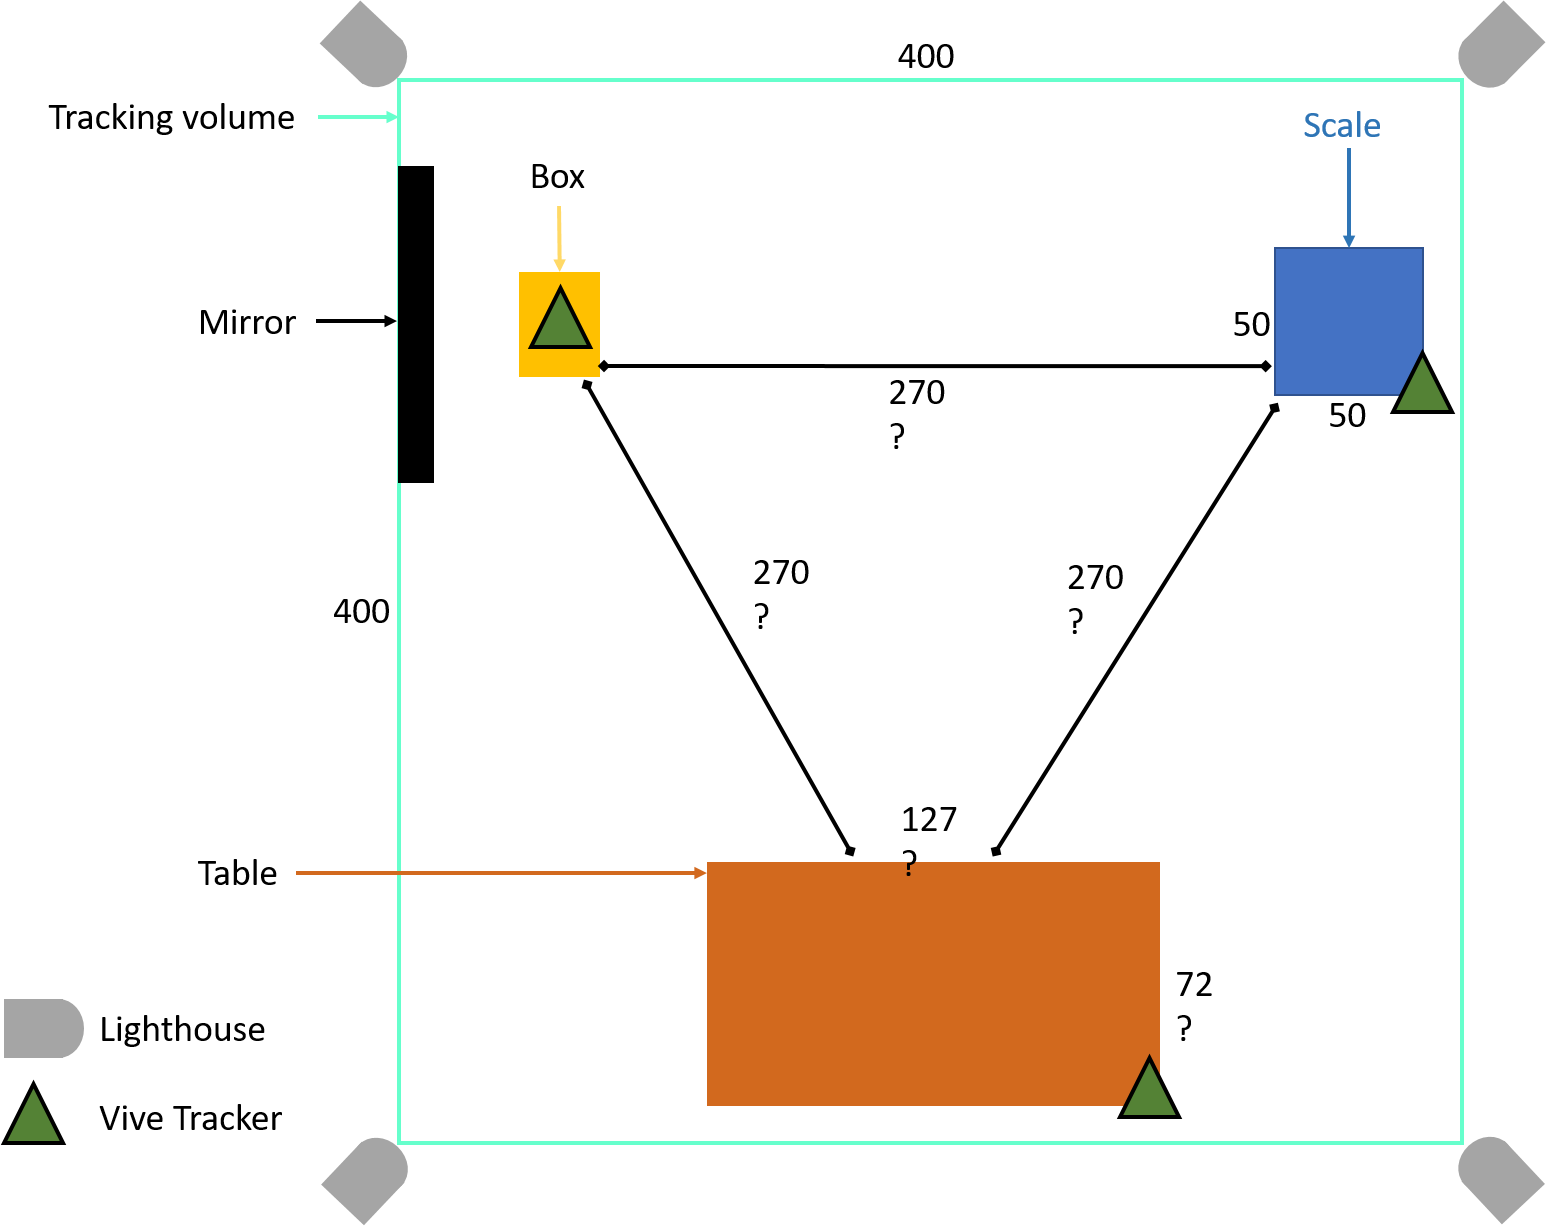
\includegraphics[width=\textwidth]{figures/study_setting.png}
	\caption[study setting]{study setting}
	\label{fig:study_setting}
\end{figure}
Meanwhile, \exgo consists out of a room, avatar representing the learner, table, box and scale. This section aims to attain an overview of the alignment of these elements. Figure~\ref{fig:study_setting} shows the real-world room in which the study is conducted. Figure~\ref{fig:learner_positions} depict all positions that are described in the task (compare table~\ref{tab:tasks}). The outer line represents the Lighthouse or tracking volume, which is approximately 400cmx400cm. On the left wall, the mirror is located. In front of the mirror, the starting and end position of the box is seated. Beside the box is the position mirror, the start and endpoint of the learner. The table is placed int the middle of the wall to the left of the mirror. Around the table, the positions table centre, table right and table left is located. At the opposite wall of the mirror, the scale is placed. In front of the scale is the position scale.
\begin{figure}[htb]
	\centering
	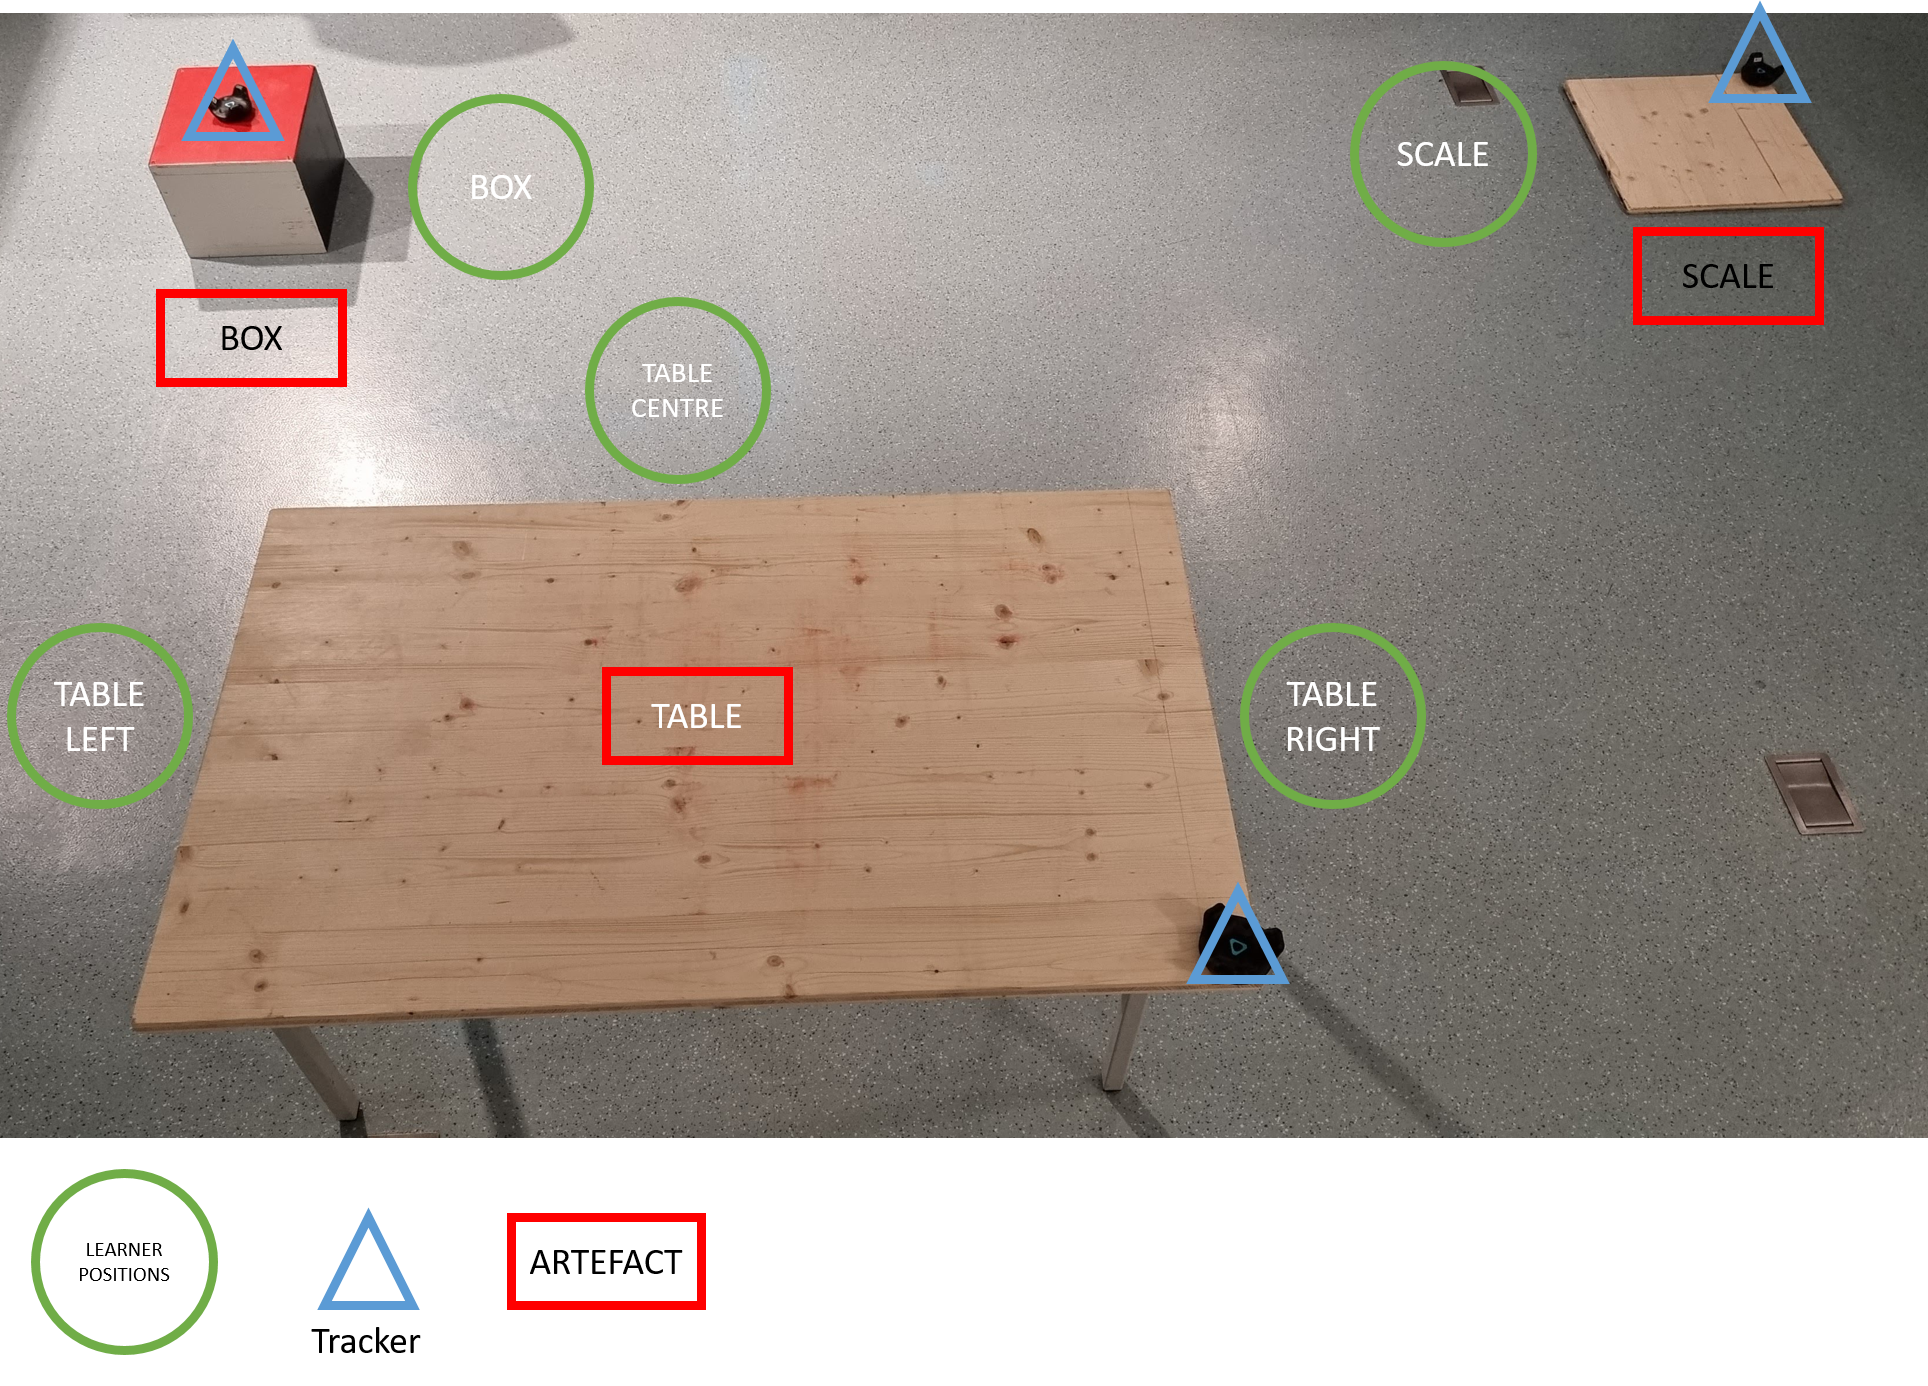
\includegraphics[width=\textwidth]{figures/learner_positions.png}
	\caption[learner positions]{learner positions}
	\label{fig:learner_positions}
\end{figure}

\subsection{Guidance Visualisation}
\label{sec:gv}
The next task is to add the GV to \exgo, which the learner can mimic. The GV is an avatar like the learner's avatar, with the difference that the motion of the GV is driven by the pre-recorded tasks 1-3. The recording of the tasks was also performed with \exgo. To use \exgo as a recorder, a copy of all trackers and the HMD is created. This recorder-copy is packed as one GameObject with the trackers as children. The parent GameObject is recorded during the performance of the movements. For the GV, a similar GameObject as the recorder is created and serves as Input for VRIK. A detailed description is given in the project report. In this section, the main points of the process are described: the recording of the movements and the resizing of the GV to the size of the learner.\\
The movements in the task have to be performed ergonomically. The measures to evaluate ergonomic movements are the RM. To serve as a strong baseline, a professional for ergonomic movements should record the movements. Because of the COVID-19 pandemic, all approaches to record the movements by a professional failed. Eventually, I were trained by a physiologist and recorded the movements by myself. The final recordings were examined by the physiologist. Overall, the movements were rated by the physiologist as "by and large correct". The back is not always straight or at the correct angle. In task 2 during a push and in task 3 during a pull, the feet are misplaced.\\
With the recording of the tasks at hand, the GV can be animated. For the ego-centric VP it is inevitable, that GV and learner having the exact same size, else the learner cannot percept the GV correctly. Furthermore, the table, box, and scale must not resize. The solution is to record two sets of object synchronised. The first set contains the objects that have to be resized, namely the GV, the second set contains objects that must not be resized, namely the box, table and scale. The recordings were synchronised by a script, the playing of the animations in \exgo, too. The resizing of the GV takes place in three steps. First, the learner and the GV are calibrated. Then the height difference is measured between the learner and GV. In the last step, FinalIK is removed from the GV, the animated GameObject containing all trackers is removed, then FinalIK reattached and calibrated. Thus the learner and the GV have the same size.


\subsection{Perspectives}
\label{sec:perspectives}
To fulfil the studies needs, the VPs have to be implemented. 

The ego-centric VP requires, besides the learner, one ego-centric GV. The learner needs to stay inside the GV. This is achieved by the speed-mechanic. The learner's distance is calculated with the help of the tracker at the hip of the learner. The hip is projected to the floor, likewise the GV hip tracker. The projection to the floor is necessary because the speed-mechanic would apply if the GV bends the knees during lift and lower. This restricts the learner's ability to perform an error: if the learner does not bend the knees during lift and lower, the GV would stop and remind the learner to bend the knees. To investigate if the learner could percept to bend the knees, the learner must be allowed to make the error. The speed-mechanic relies on the distance between the two projected points on the floor.
Additionally, the distance finds application in another functionality. In the ego-centric VP, the learner is located inside the teacher. This means that the learner's viewport is inside the head of the GV and let the learner see the inside of the GV head. This leads to distraction by the partly rendered inner head. The solution is to remove the head rendering if the distance is below $ETD_{max}$ and reinitiate the rendering above $ETD_{max}$. The rendering is removed by replacing the materials array of the head with a material array that contains only invisible materials.\\

In the exo-centric VP, four exo-centric GV are located around the learner. The positions of the exo-centric GV were determined after the task was recorded. The difficulty is to determine the proper positions of the exo-centric GVs. First, at any point in time during every task's performance, the learner must be able to see a GV by only turning the head. Secondly, the GV and the learner should not move through a table or scale of another GV. The solution to the first part in informed by Chua et al.~\cite{thaichichua}. Chua et al. chose four representation that are in front, behind, left and right. The latter proved to be impossible if the exo-centric representations should be near enough to be observed by the learner. This is a limitation of \exgo. The GV needs to be shifted to far away from the learner not to cross other GVs artefacts. In a distance in which no crossing occurs, the movements are barely visible to be mimicked correctly. The exo-centric representations were then placed in a distance that allows being observed by the learner, the GV can access all positions without standing in an artefact at that position and that the learner never crosses a table of another GV. Standing at table center: the GV to the left is shifted by two meters to the left, the GV to the right, two meters to the right. The GV in front is shifted by 1.5 meters to the front. The GV in the back is shifted 3 meters to the back. Figure~\ref{fig:multireppositions} shows the positions of the exo-centric VP. Additionally, to the exo-centric GVs a virtual copy of the student needs to be rendered. The same values shift the virtual copy of the learner. In the last VP, the ego \& exo-centric VP, the learner has an ego-centric VP and the exo-centric GV with the corresponding virtual copies of the learner. The implementation of copying the learner and the GV and shifting them to the position is rather complex and described in detail in the project report.\\
\begin{figure}[htb]
	\centering
	
\includegraphics[width=\textwidth]{figures/positions.png}
	\caption[Positions of exo-centric GVs]{shift calc}
	\label{fig:multireppositions}
\end{figure}

\subsection{Quantitative Data Aquisition}
\label{sec:logging}
\begin{table}[H]
	\centering
	
\includegraphics[width=\textwidth]{figures/logging_detail.png}
	\caption[logging detail]{Detailed overview of logs produced by \exgo\ per frame. L: learner, GV guidance visualistion, ED: euclidean distance. *head position and rotation is biased in exo-centric conditions because of multiple GV the L can focus on. **All trackers are logged for backup reasons: after the study is conducted a measurement can become interesting that was not of imporance before. With these values any measurement can be calculated post-study.}
	\label{fig:logging_detail}
\end{table}


Section~\ref{sec:measures} defined the measures that are necessary to answer the research questions. \exgo must be capable of assessing all measures. This section explains how \exgo assesses the measures. An overview of all measures is listed in table~\ref{tab:logging_detail}. Table~\ref{tab:logging_detail} lists the logging ID, a description of what the measurement is measuring, the unit in which the measurement is measured and for which research question the measurement ist assessed. The quantitative data acquisition can be divided into several classes: (i) accuracy measurements (1-5), (ii) ergonomic measurements (6), (iii) focus measurement (7) and (iv) time measurement (9). 

\subsubsection{(i) Accuracy Measurements}
The accuracy measurements assess the discrepancy between the movements of the learner and the movements of the GV. Accuracy measurements are subdivided into distance-based measures and angle-based measure. Distance-based measures rely on the Euclidean distance between the learner's body parts and the body parts of the GV. The reference point for the body part is the tracker, which is attached to the body part. The body parts are: hip, left hand, right hand, left foot, right foot, head. The distance between the learner's box and the box of the teacher is an accuracy measurement, too. Likewise the body parts, the distance between the two boxes is the Euclidean distance between the tracker of the box and the tracker of the GV. Please note, the trackers are not visible to the learner during the study. The trackers of the GV are the recorded trackers. Angle-based accuracy measurements assess the discrepancy of orientation between the body parts and box of the learner and the GV, and is measured in angle. The calculation of the angle-based measurements complies with the calculations of the distance-based measurements. This means, the angle between the corresponding trackers are measured. To conclude: distance-based measurements assess the positioning's error, angle-based measurements assess the error in orientation.

\subsubsection{(ii) Ergonomic Measurements}
The ergonomic measurements are the four risk measurements: support base, squat, upright stance, and hip-box distance. Support base is the distance between the feet. For push and pull, lift and lower, turn and fold, pick and place each a window in which the distance should be located is defined. The definition of the window is based on the movement of the person who recorded the movement. The percentage of time the learner is inside the window is the outcome of the measurement. For a better understanding, imagine the following example: the window for push and pull for the support base is 20cm-30cm. During the performance of push, the learner's feet distance was inside the window for 90 seconds. The whole performance of push lasted 100 seconds. The RM support base yields in a score of 90\%. Because the movements were recorded by myself and not by a professional, the window defined on my own movements would be missleading. Because of this predefined error, the definition of a window is renounced.\\
The measurement for squat is the distance of the hip and floor. It indicates if the learner bent the knees correctly. It is applied in the sub-tasks lift and lower. Calculations of the RM score of squat complies with the support base.\\
Upright stance is the measurement of the spine bend is correct. For upright stance, an additional tracker is applied on the back of the student, above the hip tracker. The angle of spine bend is the angle between the upright vector and the vector of the upper hip tracker. Upright stance is applied for push and pull, lift and lower, turn and fold. The bend angle during pick and place depends heavily on the box's position on the table and thereby varies. Because of this variation, a window cannot be defined for pick and place, and though the RM upright stance is not applied to pick and place. Calculations of the RM score of upright stance complies with the calculations of the preceding RM.\\
Hip-box distance is calculated by the distance between the hip tracker and the box tracker. It is applied for the sub-task carry. The calculations comply with the preceding RMs. The limitation of hip-box distance is that the measurement is influenced by the circumference of the torso of the learner. A formative test of hip-box distance was not possible due to the COVID-19 pandemic.

\subsubsection{(iii) Focus Measurement}
\label{sec:rayTrace}
The virtual room the learner sees in \exgo is filled with tables, boxes, GVs and virtual copies of the learner. To assess on what the learner is focusing during the movements, every object received a name. In every frame, raytracing is performed. The rays' origin is the HDM and expands straight forward. The name of the object first hit by the ray is written into the log file. The name is coded with the position 0-4 (see positions in firgure~\ref{fig:learner_positions}) and an object identifier (box, table, scale, GV, learner). A test revealed a systematic error by pointing too high. To correct the discrepancy, colliders of the objects were increased. The tables' and scales' collider hight is increased by 20cm. The box colliders height is doubled. The learners' and GVs' avatar were wrapped into a capsule collider with a hight 200cm of and a radius of 30cm. The values were determined by experimentation. To test the values, all sub-tasks were performed, and for any point, the object which is hit by the ray is displayed. The displayed name complied with the object in focus at nearly any point in time. Using an eye-tracker would increase the accuracy but was available.

\subsubsection{(iv) Time Measurement}
The speed of the GV animation is determined by the distance between the learner and the GV. Comparing the time the learner needed to perform the task with the time the tasks lasts without the speed-mechanic can draw conclusions about the learner's position to the GV. The tasks differ in the amount of time to be performed. The plain-times without the speed-mechanic are: task 1 takes 172128ms, task 2 189040ms and task 3 176668ms. The subtraction of the plain-time from the total time is the additional time the learner needed to perform the movement. The time discrepancy can also be applied to specific sub-tasks. This measurement will mainly be used in the evaluation for triangulation. 

\subsection{Qualitative Data Aquisition}
\label{sec:quali_logging}
The qualitative data assess during a study session relies on two questionnaires. After each condition, the participant is asked to fill the after session questionnaire (appendix A). After all conditions, the participant is interviewed. The guideline of the semi-structured interview is attached in appendix B. The questionnaires aim to assess the participant's impressions and opinions about the VPs. In the questionnaires, a different wording is applied to ease understanding. For example, the GV is called virtual teacher. 

\subsubsection{After Session Questionaire}
The after session questionnaire starts with a question about the subjective overall performance of the learner. 
\begin{itemize}
	\item[Q1:] How accurate did your movements comply with the virtual teacher?
	\item[A:] Likert scale from one (very good) to 7 (very poor)
	\item Linked research questions: RQ1.1.1-3, RQ1.4
	\item Triangulation for (1-4,6)
\end{itemize}
The answer to this question gives insights into how accurate the participant assesses the performed movements. Furthermore, this question can be used to determine if the qualitative accuracy complies with the participants' subjective opinion. The next question aims to assess the user's subjective performance for the sub-tasks. The participant is asked to fill in a table. Each line represents a sub-task. Each sub-task can be rated on a Likert scale from 1 (very good) to 7 (very poor).
\begin{itemize}
	\item[Q2:] During the task there were several smaller reoccurring movements, like pulling or lifting the box. Please rate these smaller movements, to what extend you could follow to movements.
	\item[A:] Likert scale from one (very good) to 7 (very poor) for each sub-task.
	\item Linked resarch questions: RQ1.1.1-3, RQ1.4
	\item Triangulation for (1-4,5,6)
\end{itemize}
\begin{figure}[H]
	\centering
	
\includegraphics[width=0.5\textwidth]{figures/sub-task-rating.png}
	\caption[sub task rating]{sub task rating}
	\label{fig:subtaskrating}
\end{figure}
Beside the objective opition about the participants performance, the answers of this question can be used to compare with the qualitative data. Question three aims to assess the subjective accuracy of the participants body parts.
\begin{itemize}
	\item[Q3:] Please rate to what extend you think you could align your body parts with the teachers body parts. 
	\item[A:] Likert scale from one (very good) to 7 (very poor) for each body part.
	\item Linked resarch questions: RQ1.1.1-3, RQ1.4
	\item Triangulation for (1-4,5,6)
\end{itemize} 
\begin{figure}[H]
	\centering
	
\includegraphics[width=0.5\textwidth]{figures/body-parts-acc.png}
	\caption[sub task rating]{sub task rating}
	\label{fig:bodypartsacc}
\end{figure}
This question assesses how good or bad the participant could see the body parts of the GV. The last question is not handed to the participant. It serves as the basis for a semi-structured interview. It gives the possibility to dig into extreme values of the questions answered before and in any incidences that occurred during the task's performance. Furthermore, the participant is encouraged to speak frank about the session. 
\begin{itemize}
	\item[Q4:] (As interview question) Did you have problems to follow the instructions? 
	\begin{itemize}
		\item E.g. because you could not see some body parts?
		\item E.g. bad perception related to the perspective?
		\item Go into extreme values of this questionnaire! 
		\item Address critical incidences!
	\end{itemize}
	\item[A:] Take down of participants statements.
\end{itemize}

\subsubsection{Semi-Structured Interview}
After all three sessions done, the participant is interviewed. The interview is semi-structured. The guideline contains seven main questions, partly with additional hints to dig deeper or lower the participant's entry threshold to start reporting.
\begin{itemize}
	\item[Q5:] You saw three visual perspectives: ego-centric, exo-centric and the combination. What do you think about these perspectives?
	\begin{itemize}
		\item entry question, encourage participant to talk frank, address interesting mentions
	\end{itemize}
	\item[] Linked research question: RQ1.4
	
	\item[Q6:] Prioritise the perspectives by to what extend you think you could follow the movements. (1 best to 3 worst) 	
	\begin{itemize}
		\item Why did you decide for the prioritisation?
	\end{itemize}
	\item[] Linked research question: RQ1.4
	
	\item[Q7:] Imagine you want to learn a movement in VR. Which perspective would you use for that?
	\begin{itemize}
		\item -	Or would you use a totally different one?
	\end{itemize}
	\item[] Linked research question: RQ1.4
	
	\item[Q8:] In which of the three perspectives was the easiest to understand? 
	\begin{itemize}
		\item Was there a perspective that confused you?
		\item Was there a perspective you did not understand right away?
		\begin{itemize}
			\item What do you think caused the confusion?
		\end{itemize}
	\end{itemize}
	\item[] Linked research question: RQ1.4
	
	\item[Q9:] What do you think are the advantages and disadvantages of the perspectives?
	\item[] Linked research question: RQ1.4
	
	\item[Q10:] Could you see some body parts better or worse in the perspectives?
	\begin{itemize}
		\item What about your legs, arms, back?
		\item Could you detect that during lift and lower you should squat?
		\item Could you detect that you should step back during push and pull?
	\end{itemize}
	\item[] Linked research question: RQ1.4
	
	\item[Q11:] Did you miss a feature?
	\begin{itemize}
		\item Dig for improvements for \exgo or experiment design.
	\end{itemize}
	
	\item[Q12:] (Space to ask for critical incidences if any occurred.)
\end{itemize}


\subsection{Study Procedure}
\label{sec:procedure}
As soon as the participant enters the room, the participant receives a warm welcome to feel comfortable.\\
The process starts with a Welcome letter (appendix C), followed by the informed consent and a demographic questionnaire. In the meantime, \exgo is set up by choosing the condition, set the gender of the participant as well as the log is configured with the participant ID and task id. After the demographic questionnaire, a spoken explanation about what is about to happen is given. Then the trackers are attached to the participant. The calibration process is explained: looking in the mirror and extend the arms. An explanation of the perspective is provided. Then, the first session is started. \exgo gets started, the cameras and screen recording are set up, and the participant gets the HMD. The participant is asked to stand in front of the mirror to calibrate. For calibration, the key C is pressed at the PC. To identify the camera recordings, a sign is held into the cameras. The task is started with the key S. During the session, attantion is payed to the cable of the HMD to avoid stumble of the participant. Furthermore, the participant is observed. After the session ended, the HMD is removed. The participant fills in the after session questionnaire. Session two and three are conducted likewise. After all three sessions, the trackers are removed. The participant is interviewed. The payment is given and the receipted singed. At the very end, the participant is thanked and said goodby. If it appeared, doorstep talk is appreciated.

\subsection{Limitations}
\label{sec:limitations}
\exgo and the study is designed for a task that includes the handling of physical load. If the outcome can be applied to movements without a physical load is questionable. Furthermore, the exo-centric GV sometimes walk through artefacts (table, scale) of other GV, which can confuse the study participant. The movements are not recorded by a professional, errors in ergonomic movements are possible. Lastly, only a small number of participants participated in the formative tests to evaluate partial aspects of \exgo. Especially, the hip-box distance is not tested because multiple persons with different physique would be necessary. 

box as place holder for other physical load questionabel
\chapter{Study Evaluation}
\label{chapter:study_evaluation}
\section{Study Evaluation}
\label{sec:study_evaluation}
The study presented in the last chapter is evaluated with the help of a pre-pilot study and a pilot study. The pre-pilot study was conducted with one participant and focussed on flaws in the process. Subsequently, a pilot study was cibducted with three participants. The pilot study focuss lies on the review of the \exgo\ and the assessment of data. This section describes the findings of the pilot studies and provides improvements for the actual study.

\subsection{Process}
In the beginning, the participant receives a welcome letter. Two participants stated that the information in the welcome letter about how VR headsets work is not necessary. The welcome letter was then shortened by the removal of that passage. The informed consent is signed. The following demographic questionnaire allows putting the study's data into context. During the review of the produced study data, no further questions occurred. The demographic questionnaire needs no further improvements. While the participant reads the welcome letter, the system is set up. The pilot study showed that the time to set up the system and fill in the questionnaires are corresponding.\\
Afterwards, the participant is told that he/she will be equipped with the trackers and where the trackers will be attached. Afterwards, the trackers are attached to the participant. To respect the privacy of the participant, the trackers are handed to the participant and instructions are given on how to attach them. The pilot study showed that the participants had problems following the instructions correctly. For the actual study, the participants will be asked if it is ok that the trackers are attached with the physical help of the study conductor.\\
Next, the participants received information about what to expect in the VR. The instructions contained information about the GV ("You will see one/multiple teachers.") and the task ("Please follow the instructions of the teachers as exactly as possible."). Furthermore, the participant was asked to pay attention to the ergonomics of the movements. Explanations about the speed-mechanic were provided, too ("The teacher will wait for you if you are too far away from the teacher. If that is happening, correct the placements of your feet, and it will go on."). No participant had difficulties understanding the instructions. Additionally, the participant was handed the box to get used to it before seeing its digital pendant in VR. Finally, the calibration of the system was explained ("Please look into the mirror you will see there (study conductor pointing) and extend your arms like this (study conductor performing the T-pose)"). All participants understood how to calibrate easily. The introduction of the mirror as calibration facilitator proved to be helpful and suitable.\\
Subsequently, the camera recordings were started and the participant performed the first task. In this phase of the study, two errors occurred which needed adjustments to the process. In one case, the wrong task was chosen, which made participant 1 (PT1) perform task 1 (T1) two times in different perspectives. PT1 recognised that, too. Before starting the task, an "is everything ok" checklist should be gone through. The second error regards the identification and synchronisation of the video recordings. At the ceiling, a GoPro films the scene from above. A second camera catches the scene from the side of the tracking volume. For identification, a sign held into the view of both cameras. This was forgotten twice. As an improvement, the sign should be placed beforehand in the area both cameras cover.\\
After the participant performed the first task, the participant took off the HMD and is asked to fill in the after-session questionnaire. The trackers stayed at the body of the participant. The pilot study showed that the tracker did not hinder the participants from sitting down and filling in the questionnaire. In the pilot study, a three-minute pause was conducted to allow the participant to recover. During that pause, the participant was asked about his/her wellbeing to check for VR induced motion sickness. All participants stated that they do not need a pause. The demographic questionnaire revealed that all participants were experienced with VR-system and they are used to wear VR HMDs. The pause will be maintained, because a person with no prior exposition to VR could feel different.\\
Session two and three are conducted in the same way as session one. With all three sessions done, the trackers are removed, and the semi-structured interview was conducted. Because the pilot participants were not paid, the pilot study ended here. The planned duration of the study was 75 minutes. All pilot studies took no longer than 55 minutes.  With an additional buffer, the planned study duration can be decreased by 10 minutes to 65 minutes.\\
Additionally, for the study's evaluation, the participants were interviewed to get insights about the studie's and system's flaws. The participants were asked if the explanations were sufficient and if there were any confusing elements or unclear questions in the questionnaires or documents. Finally, the participants' opinion about possible improvements of \exgo\ and the study were asked. The results of those interviews informed section~\ref{sec:studyStructure}, too.\\
To conclude, vast parts of the planned study process proved to be suitable. Adjustments are made to the welcome letter, the trackers' attachment with the study conductor's help, an additional checklist to check the session task and perspective is introduced, and the camera recording identification is improved by placing the sign into the recording area beforehand.

\subsection{\exgo}
All hardware artefacts of \exgo\ are suitable without objections. The study participants rated the box's size and weight as "okay" while still perceiving it as a "physical load". The table's size is sufficient for all three tasks. At no time, the were the participants in danger to collide with a physical artefact. The size of the scale is also sufficient. The box was always placed on the scale safely. The positions and itinerary between mirror, table and scale are without complaint. Regarding the hardware part of \exgo, the pilot study revealed two insights, one related to the trackers and one related to the HMD. The tracker at the hip is attached with a strap around the hip of the participant. While the sub-tasks \textit{lift} and \textit{lower}, the tracker is shifted upwards. The upwards shift affects the avatar's presentation and influences the accuracy measurements hip distance and the RM squat distance and upright stance. To prevent this, the student was asked to wear a belt. The tracker belt was then fixated to the participant belt with a band of velcro. This includes touching the participants in the lower hip area from behind. To prevent participants from feeling uncomfortable during the whole study, the fixation of the two belts should be performed with a clip that the participant can attach themselves. The second insight regarding the hardware of \exgo\ is the cable of the HMD. During the study, the study conductor handled the cable not to influence the participant. In one case, the cable was plugged out during a session. \exgo\ is designed for that case, and plugging in the cable again allows to continue with the session. However, in the actual study, this incident would lead to unusable data for all three sessions of that participant because, meanwhile the cable is plugged in again, the GV will move forward, and the error will be high during this phase. The actual study will benefit from a wireless HMD.\\
One participant stated that he/she could not identify the ownership of the box right away. As soon as the own box is in the participant's hands, it is no problem to tell which is the GV's box and which is the learner's box. However, if both boxes are stationary, the participant could not detect which is the own box. The box should be changed to light transparency for a better distinction between the learner's box and the GV's box. This will also have an influence on the perception of the box during \textit{lift}. During \textit{lift}, the learner's box is occluded by the GV's box for a short time. For conformity, the avatar, table and scale of the GV's should also be rendered with a light transparency.\\
The pilot study served as the last test before the actual study. An essential part of the pilot study is the review of the produced data. During the development, the measures could only be tested individually. The pilot study allowed for the first time to get a whole image. Fortunately, most of the logged data worked as intended. Only minor errors were detected. For spine bend, a last-minute edit caused an incorrect calculation. For EXO, in combination with task 2, an invisible error was detected: the props animation controller, which animates the GV's box, played the wrong task for the ego-centric GV. In EXO, the ego-centric GV is invisible but used to calculate the measurements. For EGO, the learner's avatar identification name (used for looking at, identifying what the learner is visually focussing on) is incorrect. Lastly, Unity3D natively uses comma as decimal separator. Most statistics programs natively use points as decimal separator. A log file of one session contains around 2.5 Million decimal separators. Converting a log file is time-consuming, and therefore, the logging should be changed to use a point as decimal separator.

das zeug aus den questionaires
\subsection{Qualitative Data Aquisition}
After each session, the participant fills in the after-session questionnaire. The last question of the questionnaire is not handed to the participant but asked as interview questions. The feedback of the pilot study's participant was positive, and the three questions were clear and understandable. However, during the analysis of the quantitative data, questions appeared that are worth to ask the study participants:
\begin{itemize}
	\item[Q:] How ergonomic do you think your movements have been?
	\item[A:] Likert scale from 1 (very good) - 7 (very poor)
	\item[] Linked research questions: \todo{todo}
	\item[] The self-assessment of the study participants' performance regarding the ergonomics of the movements can give insights into the participants' feelings. It is expected that the VPs with exo-centiric GVs is rated higher because the posture of the GV can be observed from the side. For example, the back of the GV's bend angle is hard to see in the ego-centric VP. Furthermore, the self-assessment can be put into relation to the quantitative data and used for triangulation.
	\item[Q:] On what did you focus most?
	\item[A:] Two choices: box, teacher
	\item[] Linked research questions: \todo{todo}
	\item[] The assessment of the subjective participants' focus can give insights about the importance of box and avatar for the participants. Presumably, a participant who rates the box over the avatar focussed mainly on the box's accuracy and vice versa. This subjective data can be put into relation to the quantitative data for triangulation. If the quantitative data complies with the qualitative data, the evaluation of the risk metrics can be split into two groups: those who focussed mainly on the box and those who focussed mainly on the avatar. It could be interesting if these two groups score differently regarding the risk metrics.
	\item[Q:] Could you see a teacher at any point in time?
	\item[A:] Two choices: yes, no
	\item[] Linked research questions: none, evaluation of the positions of the GVs
	\item[] The positions of the GVs could only be tested sparsely. This question aims to evaluate if the positions of the GVs were suitable. If the participant crosses "no" during the last interview question this can be addressed in the next question.
\end{itemize}
After all three sessions, the participant is a semi-structured interview. The guideline for the semi-structured interview proved to be suitable. However, during the interviews, one participant could not give a clear prioritisation of which perspective he/she would use if he/she had the choice. I gave in and did not insist on the prioritisation. This caused an inconsistency which becomes clear during the analysis of the qualitative data. In the study, every participant should provide a prioritisation.


\subsection{Acclimatisation Phase}
The first session of each study is the acclimatisation phase, where the learner gets used to \exgo. It is assumed that the learning effect between session one and two is high, and between two and three, nearly no learning effect occurs. To evaluate if this assumption holds, the task completion time (TCT) could give insights because of the \textit{speed mechanic}. The \textit{speed mechanic} regulates the GV animation speed based on the distance between learner and GV and is applied in all perspectives. The higher the learner-GV distance, the lower the speed. A learner who is often located near to the ideal point yields a lower TCT. A formative test in which one participant does the same task in all condition would lead to insights about the learning effect. Such a test was not possible because of the COVID-19 pandemic. Nevertheless, comparing the TCT in the pilot test could at least indicate if the learning effect between session two and three is low by showing similar TCT.\\
Figure~\ref{fig:tct} shows the amount of ms the participants needed more to complete the task compared with the task norm duration (over task norm duration (OTND)). The task norm time is the amount of ms the task needs to complete without the speed-mechanic. The order of the sessions is from left to right. Participant 1 (PT1) had a nearly equal OTND for all three tasks. Because of a mistake in choosing the pilot study task, PT1 faced T1 two times. However, in session three, the OTNT is slightly higher. PT2 shows the expected behaviour, having a high OTND in the first session and a nearly equal OTND for session two and three. PT3's OTND is strictly monotonically decreasing. If the OTNT behaviour of all the participants would be like PT2's behaviour, the choice of the acclimatisation method is correct. If the OTNT behaviour for all participants would look like PT3, the acclimatisation method would be incorrect. In this case a seperate condtition specific acclimatisation before every session should be conducted. Unfortunately, the data is ambiguous and does not allow an evaluation of the acclimatisation method. Thereby, using the first session for acclimatisation is maintained.


\begin{figure}[htb]
	\centering
	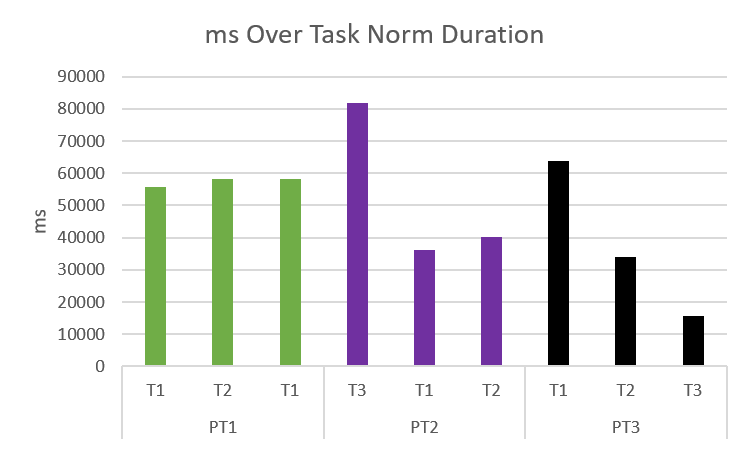
\includegraphics[width=0.8\textwidth]{figures/msOverTaskNorm.png}
	\caption[TCT of all sessions.]{Amount of miliseconds over task norm time (task duration without speed mechanic). PT - participant, T - task.}
	\label{fig:tct}
\end{figure}

\section{Data Analysis}
Based on the pilot study, this section tries to give a first glimpse of the data. The data relies on only three participants. Additionally, the data relies on a pilot study. A pilot study serves to identify issues and faults in the system and study and prepare the final study conduction. Section\todo{55} describes found issues and faults and the solution for them. Some issues and faults impacted the data, which led to the exclusion of corresponding data. Furthermore, as described in section~\ref{sec:studyStructure}, a full counterbalancing of tasks and conditions is possible with nine participants. Additionally, the data revealed, in some aspects, a high variation in both qualitative and quantitative data. Therefore, the depicted data is a rough estimation, and conclusions can not be drawn. The analysis is superficial, and a detailed analysis like significant verification is renounced. However, the first impression of a possible outcome can be given. All charts depicted in this section are similarly structured. The conditions in all charts have the same colour coding: \textcolor{blue}{EGO} is depicted in blue, \textcolor{orange}{EXO} is depicted in orange and the combination \textcolor{gray}{EGO \& EXO} is depicted in gray. For all charts (except for head angle) holds: the lower the bar, the better in the corresponding context.\\
Figure~\ref{fig:cumulatedError} can be perceived as an abstract for this section by showing the overall error in distance and angle between the learner and the GV per VP. Overall, the ego-centric VP mostly outperformed both the exo-centric VP and the ego \& exo-centric VP, while the ego \& exo-centric VP mostly scored better than the exo-centric VP.
\begin{figure}[htb]
	\centering
	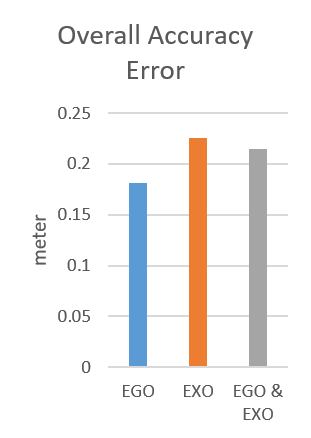
\includegraphics[width=0.3\textwidth]{figures/cumulatedDistanceError.png}
	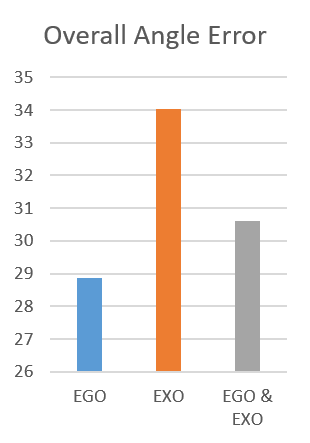
\includegraphics[width=0.3\textwidth]{figures/cumulatedAngleError.png}
	\caption[Cumulated error per perspective.]{Cumulated average distance error (left) and angle error (right) per VP.}
	\label{fig:cumulatedError}
\end{figure}


\subsection{Accuracy}
Accuracy is clustered by distance and angle and applied for the body parts hands, feet, hip, head and box. Distance is the Euclidean distance between the learners, e.g. hand and the GV hand in meters, and describes the difference in position. Angle describes the difference in orientation and is measured in degrees. The overall error per body is depicted in~\ref{fig:overallError}.
Section~\ref{sec:studyStructure} showed that some sub-tasks could be paired up, based on the similarity of the movements: \textit{lift}/\textit{lower}, \textit{push}/\textit{pull}, \textit{turn}/\textit{fold} and \textit{pick}/\textit{place}. Figure~\ref{fig:avgErrorPerSubTask} shows the average error in distance and angle per sub-task and confirms the pairing of the sub-tasks by showing a relation between the pairs. Hence, in the following, the pairs of sub-tasks will be analysed in combination. \textit{Carry} and \textit{walk} are analysed seperately. The sub-tasks structure this section. The sub-task is analysed based on the accuracy measurements and compared with the subjective accuracy of the learner.
\begin{figure}[H]
	\centering
	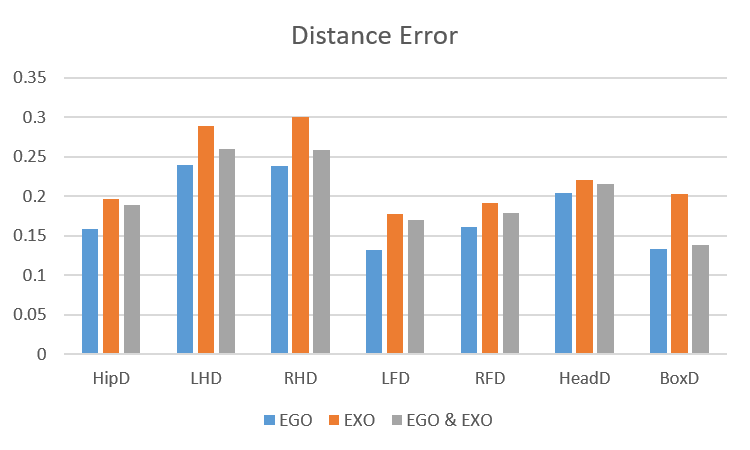
\includegraphics[width=0.49\textwidth]{figures/overallDistanceError.png}
	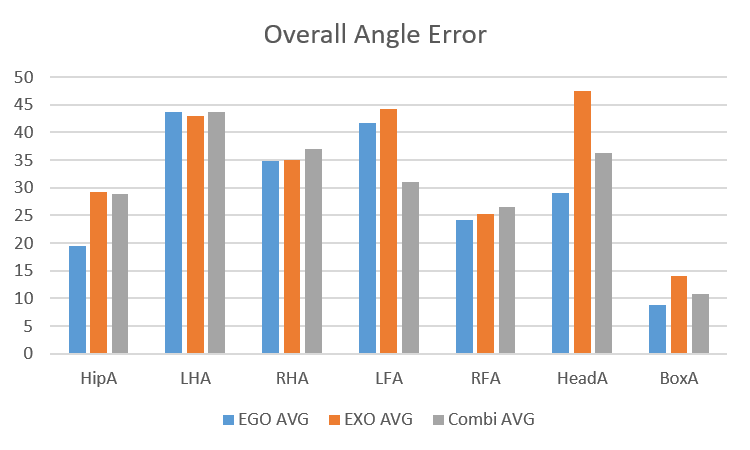
\includegraphics[width=0.49\textwidth]{figures/overallAngleError.png}
	\caption[Average error per body part in meter.]{Average error per body part. Left: distance error, right: angle error. Suffix D: distance, suffix A: angle. LH - left hand, RH - right hand, LF - left foot, RF - right foot.}
	\label{fig:overallError}
\end{figure}
\begin{figure}[H]
	\centering
	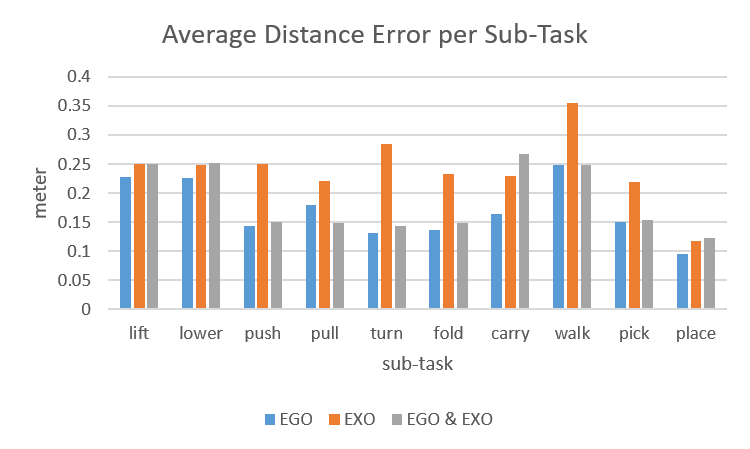
\includegraphics[width=0.49\textwidth]{figures/averageDistanceErrorPerSubTask.png}
	\includegraphics[width=0.49\textwidth]{figures/averageAngleErrorPerSubTask.png}
	\caption[Average error of sub-task\textit{carry}]{Average error of sub-task \textit{carry}. Left: distance error, right: angle error. Suffix D: distance, suffix A: angle. LH - left hand, RH - right hand, LF - left foot, RF - right foot.}
	\label{fig:avgErrorPerSubTask}
\end{figure}

Figure~\ref{fig:overallError} shows that the distance error of hands and the error of feet are related. This is expected since large parts have synchronised movements. For example, the hands touch the box simultaneously. Across all conditions, the feet's error is lower than the hands' error. The hands' error is lower in EGO than in EXO. Hands are directly visible in front of the learner and the direct comparison to the ego-centric GV is a possible explanation. Surprisingly, feet's error is lower in EGO, too. To see the feet, the learner must actively move the head, primarily if the box blocks the view on the feet. However, it seems easier to align the learner's feet with the GV feet in EGO. The box distance and angle error are lower in EGO and \combi. The presence of an ego-centric GV box increases the distance and angle accuracy for the box presumably significantly. The hip error indicates to what extend the learner could determine the correct location. The data indicates that the determination of one's own position and rotation is more straightforward with an ego-centric GV. The head angle is not comparable with the other accuracy measures. The presence of multiple exo-centric GVs in the EXO forces the learner to look into different directions. The difference between EXO and \combi\ could point out that the learner focussed in \combi\ on both the exo-centric GVs and ego-centric GV. The angle-based accuracy for the hand and feet reveal no clear trend. More participants are needed to get a clearer view. Overall, the presence of an ego-centric GV increases the distance accuracy for all body parts. For the box-shaped physical load, the presence of an ego-centric GV increases the angle accuracy, too. On the one hand, adding exo-centric GVs to the ego-centric GV decreases the distance accuracy. A possible reason could be that the learner shares the focus with multiple GVs or that the presence of four exo-centric GVs overwhelms the learner. The study participants rated their overall accuracy highest in EGO and lowest in \combi, compare~\ref{fig:overallSubjectiveAccuracy} (left). The low subjective accuracy in \combi\ would underpin the theory that the learners were overwhelmed. However, when the participants were asked about their subjective accuracy for the body parts, arms, legs and back, a different picture arises, compare~\ref{fig:overallSubjectiveAccuracy} (left). The participants' opinion is differentiated, which causes a high standard deviation of around 1.5 on a Likert scale from 1-7. More participants could lead to a clearer view. On the other hand, adding an ego-centric GV to exo-centric GVs increases the accuracy slightly.\\
The described insights rely on the whole task containing all sub-tasks. The drawn deductions are only valid for a task that includes all sub-tasks in the same amount. Potentially, the accuracy in specific sub-tasks could differ from the overall accuracy. In the following, the sub-tasks are analysed and vetted if the deductions count for the specific sub-tasks.
\begin{figure}[H]
	\centering
	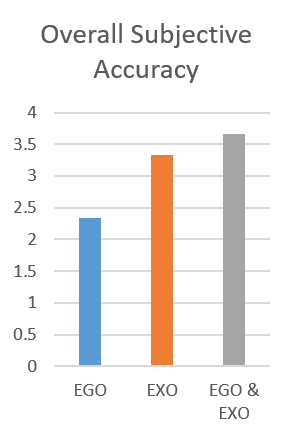
\includegraphics[width=0.3\textwidth]{figures/overallSubjectiveAccuracy.png}\\ 
	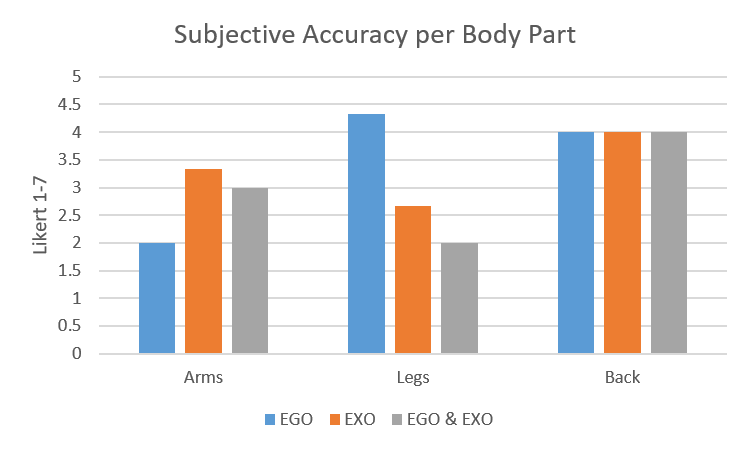
\includegraphics[width=0.49\textwidth]{figures/subjectiveAccuracyPerBodyPart.png}
	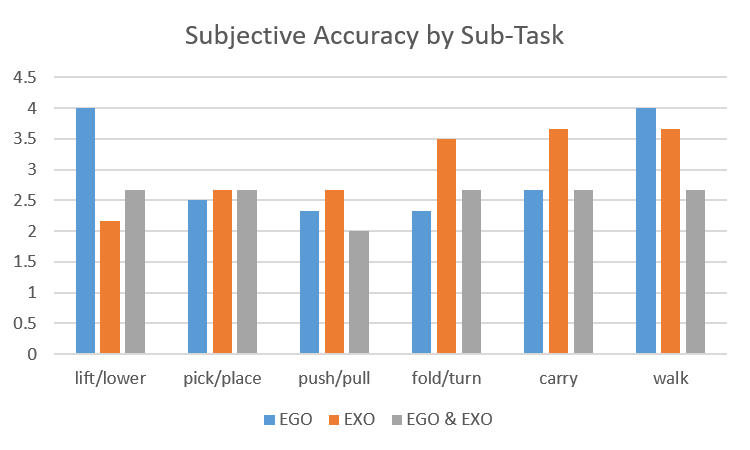
\includegraphics[width=0.49\textwidth]{figures/subjectiveAccuracyBySubTask.png}
	\caption[Subjective accuracy per VP]{Subjective accuracy per VP}
	\label{fig:overallSubjectiveAccuracy}
\end{figure}

\begin{figure}[H]
	\centering
	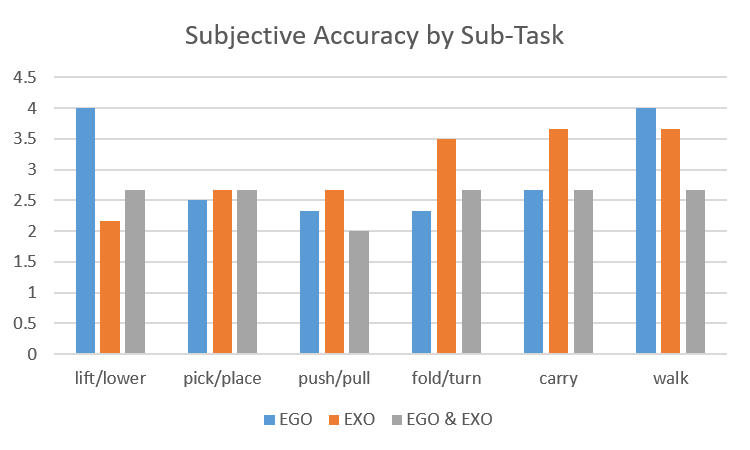
\includegraphics[width=0.29\textwidth]{figures/subjectiveAccuracyBySubTask.png}
	\caption[Subjective accuracy per sub-task]{Subjective accuracy per sub-task}
	\label{fig:subjectiveAccuracybySubTask}
\end{figure}

\subsection{lift/lower}
\begin{figure}[H]
	\centering
	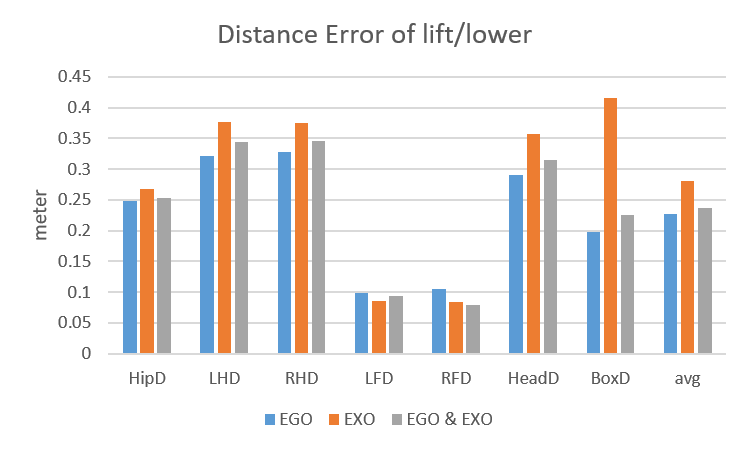
\includegraphics[width=0.49\textwidth]{figures/distanceErrorLiftLower.png}
	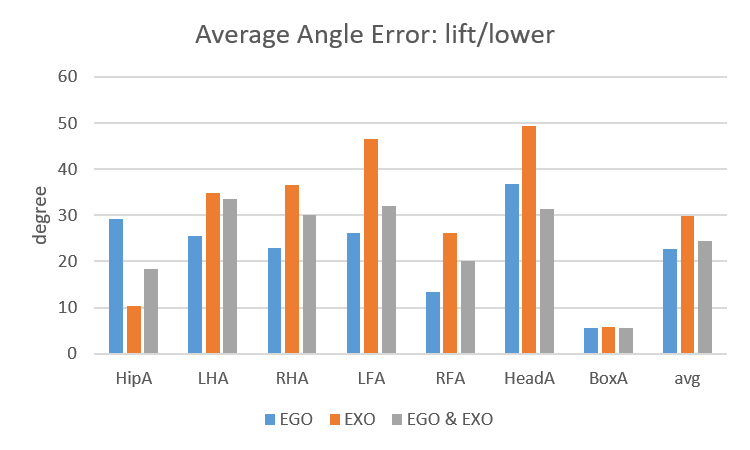
\includegraphics[width=0.49\textwidth]{figures/angleErrorLiftLower.png}
	\caption[Average error per body part for sub-tasks \textit{lift}/\textit{lower}.]{Average error per body part for sub-tasks \textit{lift}/\textit{lower}. Left: distance error, right: angle error. Suffix D: distance, suffix A: angle. LH - left hand, RH - right hand, LF - left foot, RF - right foot.}
	\label{fig:errorLiftLower}
\end{figure}
Figure~\ref{fig:errorLiftLower} shows that in EGO, the hip, hand and head accuracy is higher than in an EXO. The presence of exo-centric GV seems to have a positive influence on the feet's accuracy. The box's accuracy in EXO is lower than in EGO and EXO. In the actual study, particular attention should be paid to the box during \textit{lift} and \textit{lower} to identify the cause of why EXO performed badly. In orientation, the box's error is low for all VPs. This is expected since the sub-task does not include a change in orientation.
The subjective accuracy is by far lowest in EGO, followed by EGO and EXO.

\subsection{pick/place}
\begin{figure}[H]
	\centering
	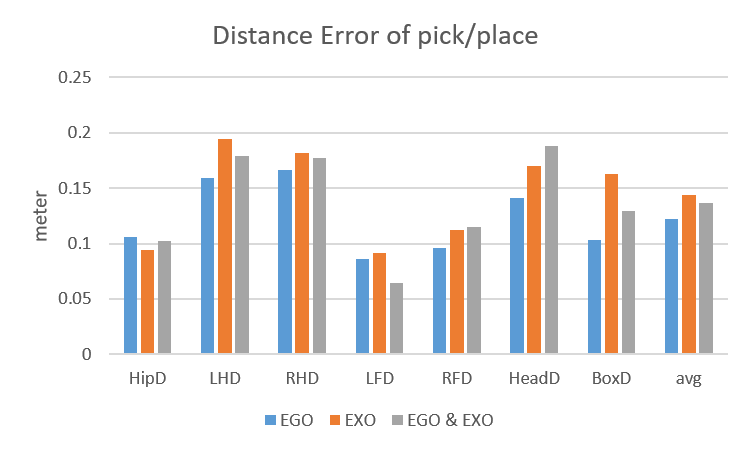
\includegraphics[width=0.49\textwidth]{figures/distanceErrorPickPlace.png}
	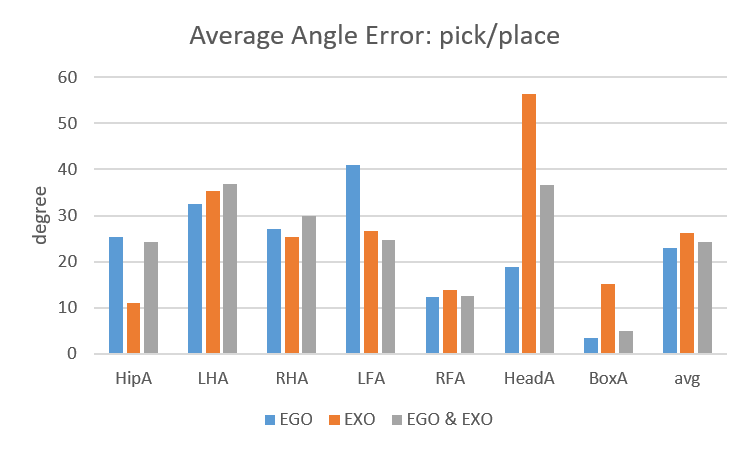
\includegraphics[width=0.49\textwidth]{figures/angleErrorPickPlace.png}
	\caption[Average error per body part for sub-task \textit{turn}/\textit{fold}.]{Average error per body part for sub-task \textit{turn}/\textit{fold}. Left: distance error, right: angle error. Suffix D: distance, suffix A: angle. LH - left hand, RH - right hand, LF - left foot, RF - right foot.}
	\label{fig:errorPickPlace}
\end{figure}
\textit{Pick} and \textit{place} are \textit{lift} and \textit{lower} movements with a significant difference in magnitude. The accuracy of pick and place benefits from the presence of an ego-centric GV. The distance and angle error of the box is lowest in EGO.
\subsection{push/pull}
\begin{figure}[H]
	\centering
	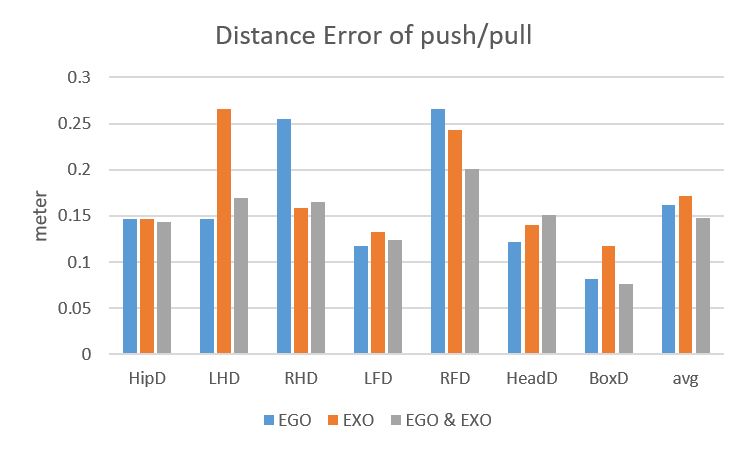
\includegraphics[width=0.49\textwidth]{figures/distanceErrorPushPull.png}
	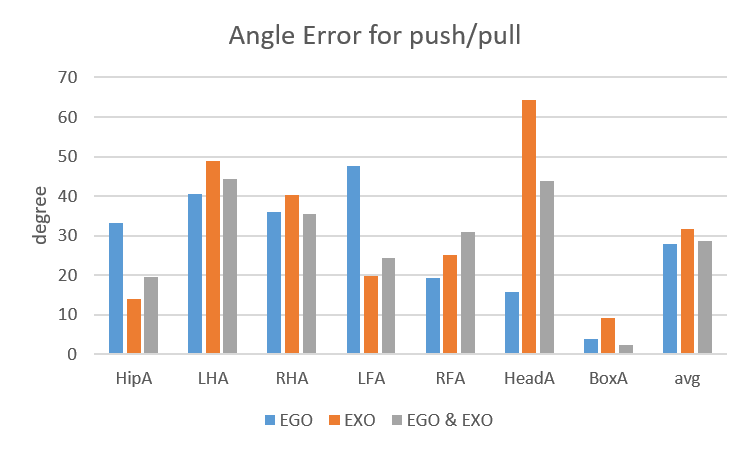
\includegraphics[width=0.49\textwidth]{figures/angleErrorPushPull.png}
	\caption[Average error per body part for sub-tasks \textit{push}/\textit{pull}.]{Average error per body part for sub-tasks \textit{push}/\textit{pull}. Left: distance error, right: angle error. Suffix D: distance, suffix A: angle. LH - left hand, RH - right hand, LF - left foot, RF - right foot.}
	\label{fig:errorPushPull}
\end{figure}
During \textit{push} and \textit{pull}, increased force is applied to the box. The physiologist suggested that one foot should be shifted to the back for \textit{push} and \textit{pull} because of the increased force application. The high difference in error between the left foot and right foot is based on different foot placement. Unfortunately, the participants realised the different foot placement not often. One participant stated that he did not realise to shift one foot back in EGO in the interview. However, in EXO, he saw it and applied it then also for \combi. This statement harmonises with the quantitative data, which shows the lowest accuracy in EGO. The left hand seems to have a high error in EXO, the right hand in EGO. The video revealed that the participants alternated the hand placement during \textit{push} and \textit{pull}. Based on the video observation, the high error could even out with more participants. The higher error of the head angle in EXO compared to \combi\ indicates that the participants shared the focus in \combi\ with the ego-centric GV and the exo-centric GV. The participants rated their movements more exact in \combi\ than in EGO and lowest in EXO.

\subsection{turn/fold}
\begin{figure}[H]
	\centering
	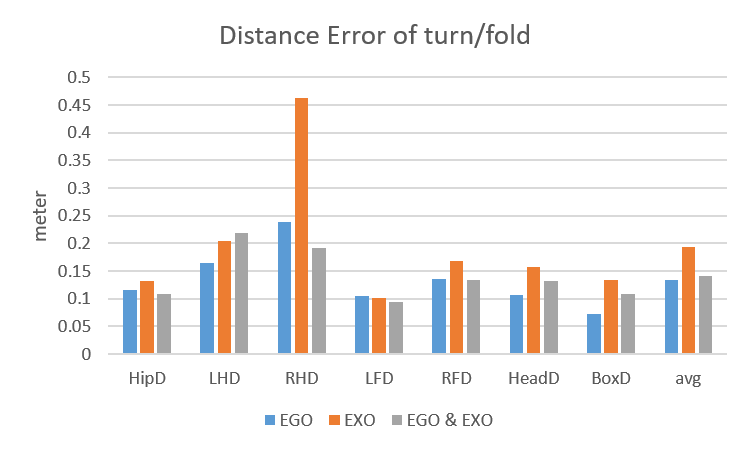
\includegraphics[width=0.49\textwidth]{figures/distanceErrorTurnFold.png}
	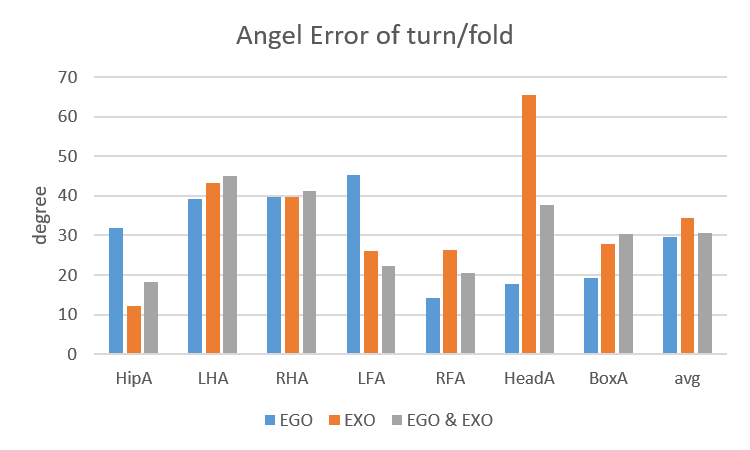
\includegraphics[width=0.49\textwidth]{figures/angleErrorTurnFold.png}
	\caption[Average error per body part for sub-task \textit{turn}/\textit{fold}.]{Average error per body part for sub-task \textit{turn}/\textit{fold}. Left: distance error, right: angle error. Suffix D: distance, suffix A: angle. LH - left hand, RH - right hand, LF - left foot, RF - right foot.}
	\label{fig:errorTurnFold}
\end{figure}
Most of the movements during \textit{turn} and \textit{fold} happened on the table. Thus the main focus is on the hands. The high error in EXO is noticeable. The consultation of the video recordings revealed that in EXO, the participants could not see the direction of \textit{turn} directly and changed the right hand after the movement began. Furthermore, after starting to \textit{turn} or \textit{fold} the box, the participants changed the hand's position, presumably to ease the movement. The perceived accuracy is highest in EGO, followed by \combi\ and EXO. 

\subsection{carry and walk}
\begin{figure}[htb]
	\centering
	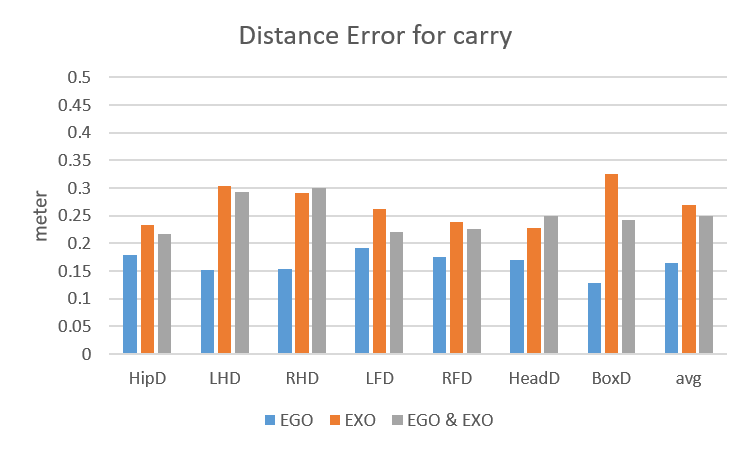
\includegraphics[width=0.49\textwidth]{figures/distanceErrorCarry.png}
	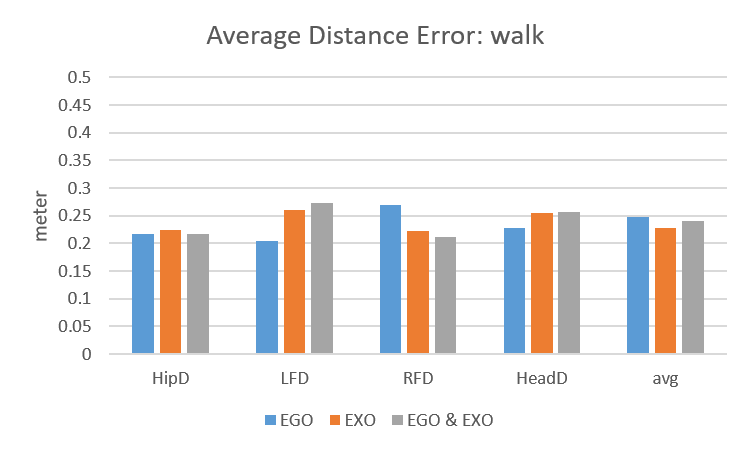
\includegraphics[width=0.49\textwidth]{figures/distanceErrorWalk.png}
	\caption[Average error of sub-tasks \textit{carry} and \textit{walk}]{Average error of sub-tasks  \textit{carry} (left) and \textit{walk} (right). Suffix D: distance. LH - left hand, RH - right hand, LF - left foot, RF - right foot.}
	\label{fig:walkError}
\end{figure}
Teaching locomotion in the ego-centric VP with the help of the \textit{speed mechanic} is a novelty. The data revealed a nearly equal error for ego-centric guided walking and exo-centric guided walking. The position of the hands are not essential for walking and are not depicted. Adding a physical load to walking (\textit{carry}) has a strong influence on accuracy. The learner seems to focus on the box and tries to match the GV's box with the own box. This increases the accuracy of their own position for all body parts.

\section{Visual Focus}
In EGO, the learner is provided one ego-centric GV and will focus on it. If exo-centric GVs are added to the scene, the learner can focus on multiple GVs. Furthermore, it is interesting which percentage of time the learner focuses on the own/GVs box and own/GVs body.\\
\begin{figure}[htb]
	\centering
	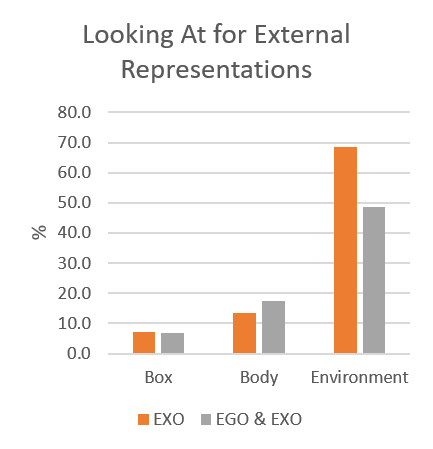
\includegraphics[width=0.5\textwidth]{figures/lookingAtExternalRepresentations.png}
	\caption[Looking At for external representations.]{When looking at an external representation, percentage of time focussing on the box or table.}
	\label{fig:lookingAtExternal}
\end{figure}
A pilot study helps to evaluate the experiment design and data acquisition. Conducting a pilot study before the actual study is vital. The proof is depicted in figure~\ref{fig:lookingAtExternal}. In section~\ref{sec:rayTrace} it is described how the looking at data acquisition method was developed and tested. The formative test was conducted with one person\footnote{More participants were not possible because of the COVID-19 pandemic.}, which is too little. The study data revealed that the data acquisition for looking at is not working correctly. Over 50\% of the time, the ray traces hit the environment. For the actual study, the artefacts and avatars' colliders should be adjusted, or if available, an eye-tracker should be used. Nevertheless, assuming the rays which hit something other than the environment are evenly distributed, some deductions can be made from the acquired data.\\
Figure~\ref{fig:lookingAtExternal} shows the percentage of time the learner focussed on the box, a body (avatar) and the environment. The learner focussed roughly twice as much on a body than on the box.\\
Figure~\ref{fig:posHeatMap} shows the positions of the GVs whereby a GV is the union of body, table and box. The positions are overlayed with a heat map. The orange circles stand for the percentage of time the learner focuses on that position. The heat map provides two insights. First, the presence of an ego-centric GV influences the visual focus of the learner. In EXO, where no ego-centric GV is present, the learner focused 11\% of the time on the own table and box. In \combi, the learner focussed 45\% of the time on the ego-centric GV. If an ego-centric GV is present, it is more frequently focussed than exo-centric GVs. By implication, the learner is consulting the exo-centric GVs, if an ego-centric GV is present.
The second insight regards position four. In EXO and \combi, the learner did not focus on the GV at position four. Position four is superfluous for all three tasks.
\begin{figure}[htb]
	\centering
	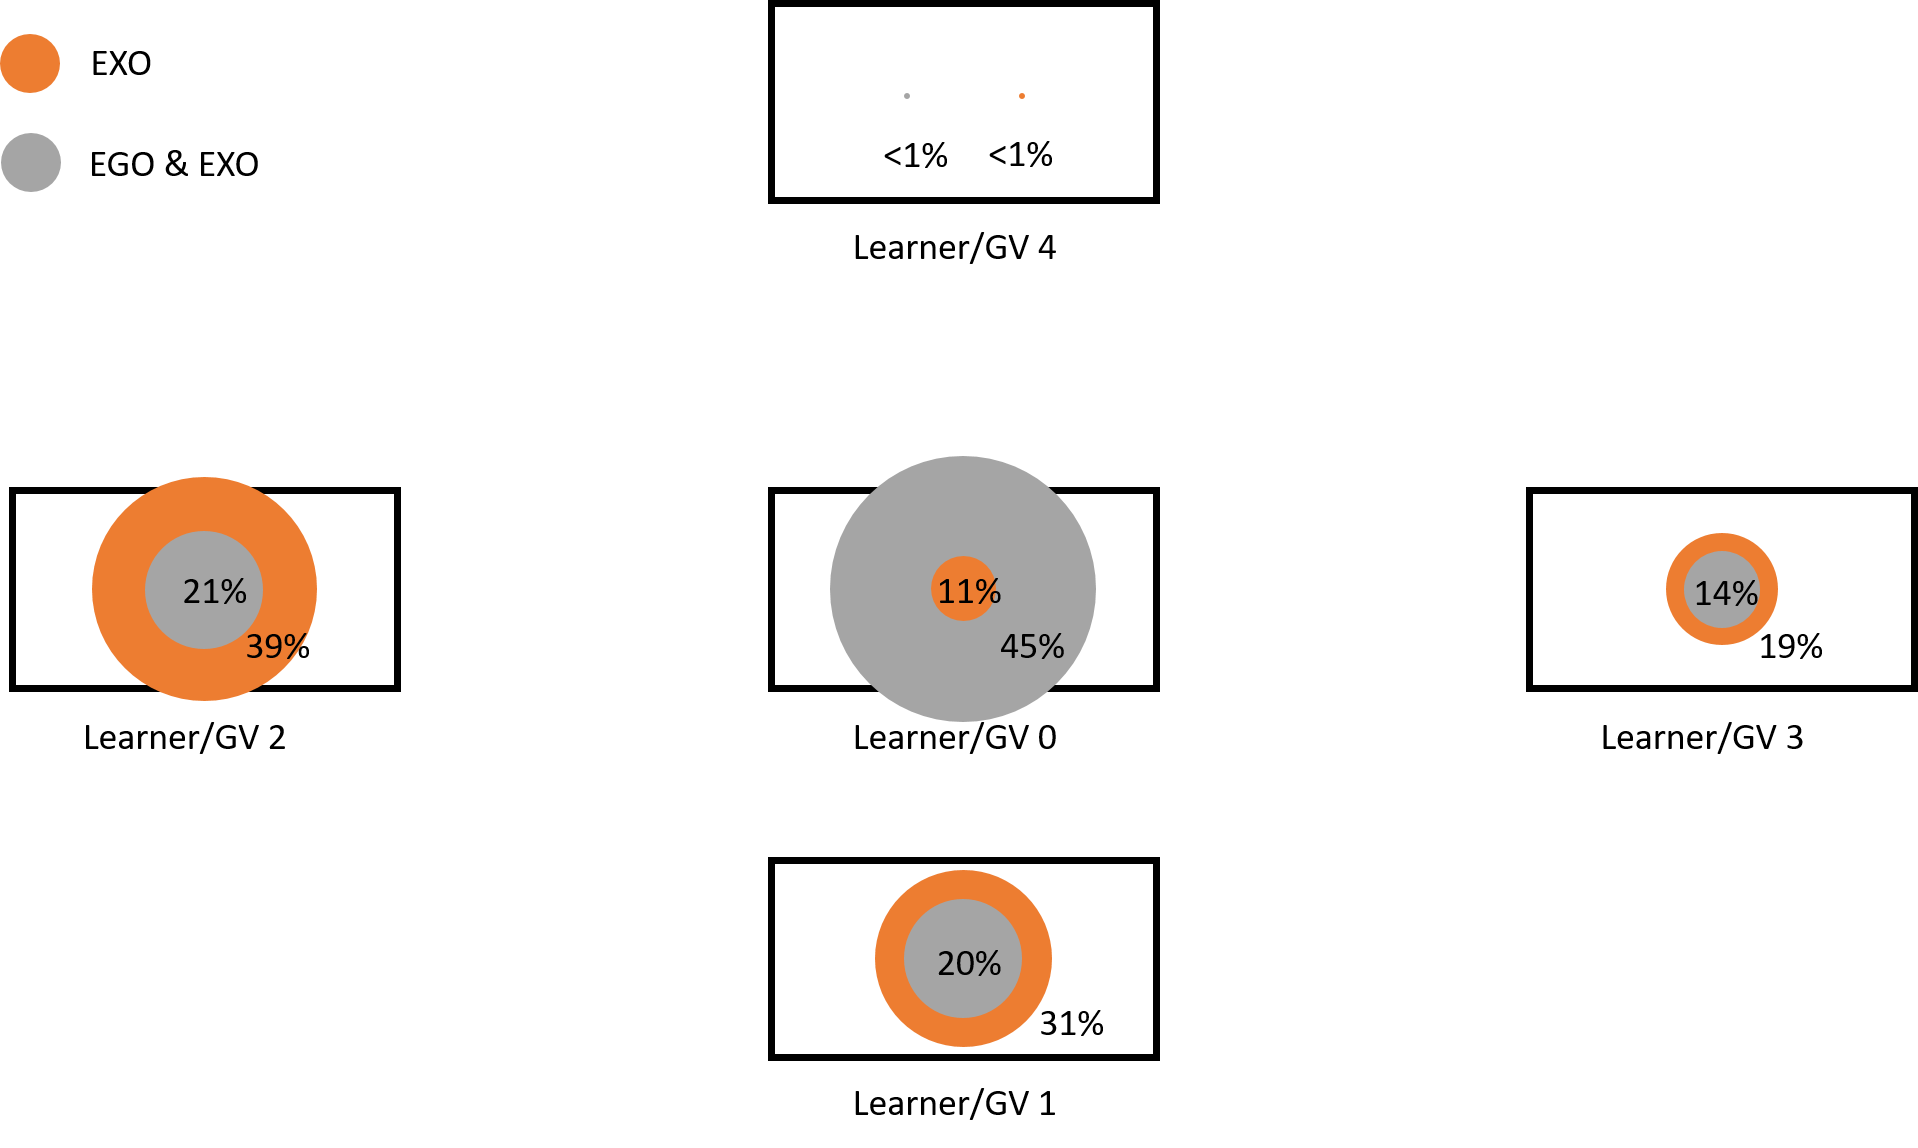
\includegraphics[width=\textwidth]{figures/positionHeatMap.png}
	\caption[\textit{Looking at} heat map.]{Heat map of the learner's focus in EXO and EGO \& EXO. The heatmap shows the tables of the multiple representations. The circles' size corresponds to the amount of time the learner focussed the representation.}
	\label{fig:posHeatMap}
\end{figure}
\todo{perceived acc per body part}

\section{Risk Metrics}
The risk metrics are not analysed. The reason refers to the missing windows the RMs are based on. Recap: for specific sub-tasks the specific RM should be between a minimum and a maximum. The time inside and outside the window between the minimum and maximum yield a score. To determine a window fo the RM a professional should be consulted. Because of the COVID-19 pandemic, a determination by a professional was not possible.\\
However, the accuracy data for \textit{lift} and \textit{lower} could lead to a guess to squat distance performance. The feet accuracy is higher in EXO than in EXO. Squat distance refers to the same body part. Thereby, the assumption seems legit that squat distance could be better in perspectives with an exo-centric GV. Good Base and Spine Bend are referring to body parts that are not directly visible in EGO, though the assumption could be extended to Good Base and Spine Bend, too.

\section{Subjective Preferences}
The personal preferences of the participants tend towards perspectives with exo-centric GVs. If the participants had chosen a VP for the task, two participants would decide for \combi, and one would use EXO. Additionally, two participants stated that they could follow the GV best in \combi, one could follow the GV best in EGO. All but one participant ranked the ability to follow the GV worst in EGO. This competes with the accuracy, which is the lowest in EGO. Surprisingly, all participants stated that the most accessible VP was EGO. In EGO, the GV stands inside the own body, which is not possible in real-world scenarios. Limitation for the ease of understanding is the high proficiency and knowledge about VR of all participants.

\chapter{Conclusion}
\label{chapter:conclusion}
(3 pages)
\section{System and Study}
Zusammenfassung der Evaluation des Systems über die eignung zur durchführung einer Studie die daten generiert um die Forschungsfrage zu beantworten.\\
Zusammenfassung was gut und schlecht ist bei der Studienausführung.\\
reflexion und contribution, inkl. zu erwartende empirische contribution\\
\section{Outlook}
\label{section:study_improvements}
Was kann noch evaluiert werden mit diesem system?\\
anderer task ohne physical load, sitzend zur bedienung von maschinen ,realismusgrad der avatare, anzahl avatare, position von avataren, geschwindigkeit der anleitungsanimation...\\
wer hat welchen nutzen von der beantwortung der forschungsfrage: designer von motorlearning vr systemen.\\
bezug zu erweiterungen der implementierung\\
possible improvement: DTW https://towardsdatascience.com/dynamic-time-warping-3933f25fcdd\\

limitations:
- nur für elementar tasks mit der bestimmten magnutude. bewegungen oberhalb oder unterhalb auch nicht passend. 
\chapter{Attachments}

\section{Learner Rendering Pipeline}
\label{a:studentRenderingPipeline}
\begin{figure}[H]
	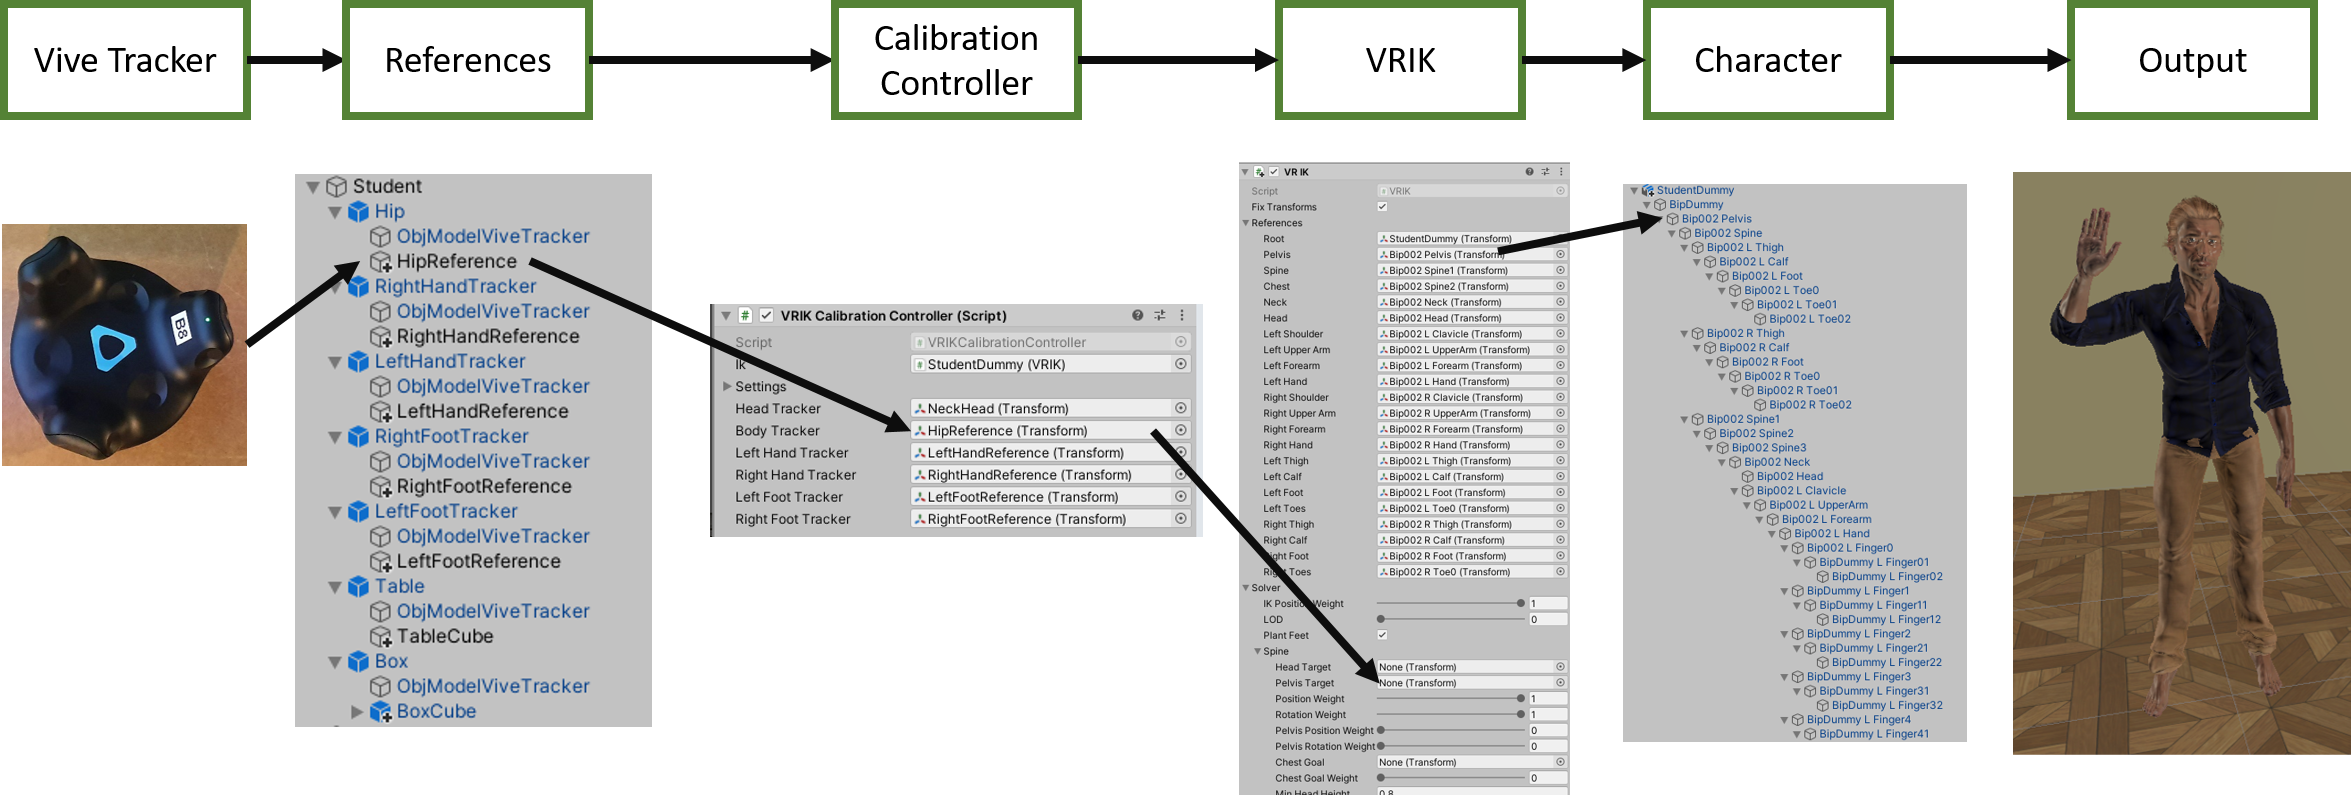
\includegraphics[angle=90,height=18cm]{figures/studentRenderingPipeline.png}
\end{figure}

\newpage
\section{Study Documents}
%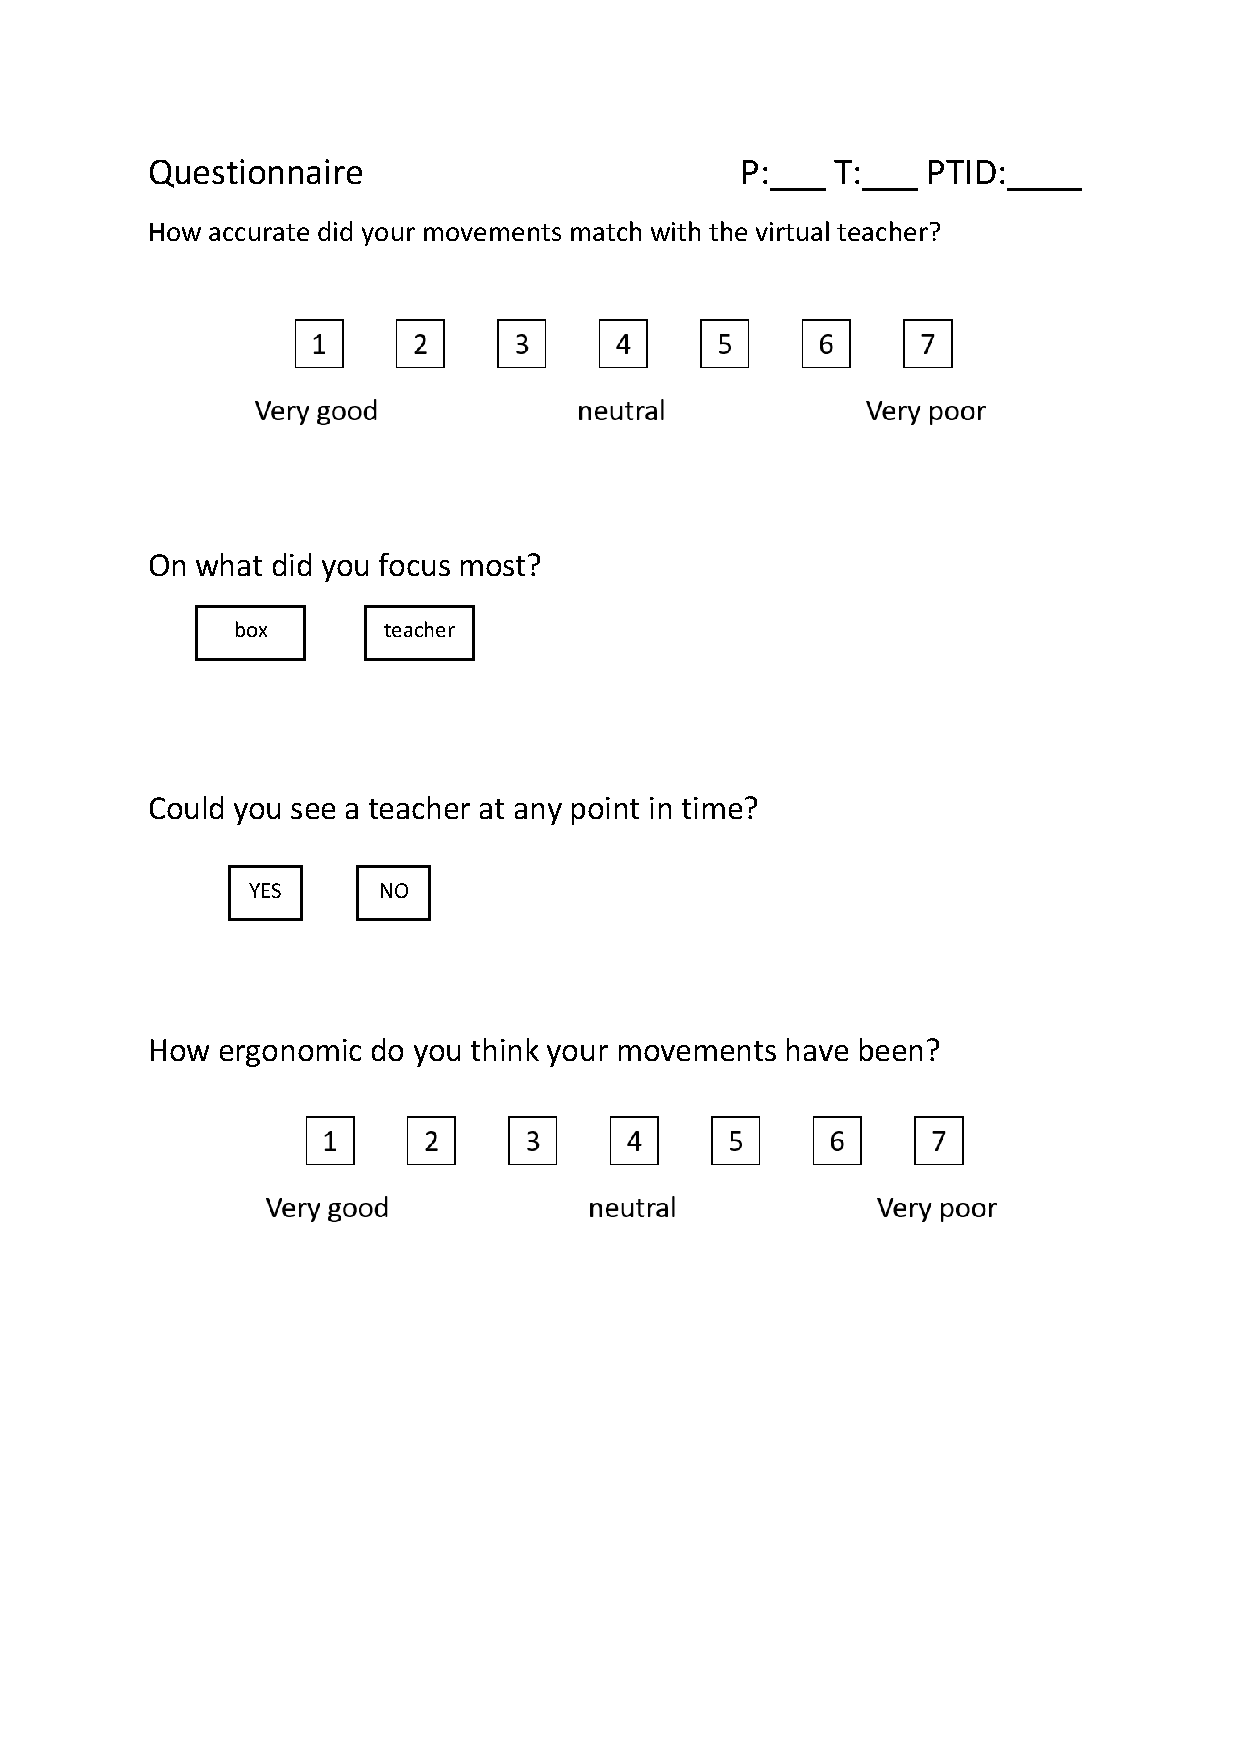
\includepdf[pages=-]{attachments/after_session_questionaire.pdf}
\begin{table}[]
	\begin{tabularx}{\textwidth}{@{}X|XXXXXX@{}}
		\toprule
		& Tai Chi Trainer \cite{thaichichua}   & YouMove \cite{YouMove} & VR Dance Trainer \cite{vrdancetrainer} & OneBody \cite{onebody} & LightGuide \cite{lightguide} & Physio@ Home \cite{physioathome} \\ \midrule
		Perspective &
		Exo-centric,\newline Ego \& augmented exo-centric &
		Exo-centric &
		Exo-centric &
		Ego-centric,\newline exo-centric &
		Ego-centric,\newline exo-centric &
		Exo-centric \\ 
		Task & Tai Chi & Dance (Ballet), abstract & Dance (HipHop)   & Martial Arts         & Abstract   & Shoulder rehab \\ 
		GV   & Avatar, \newline wireframe & Stick figure,\newline avatar     & Avatar           & Stick figure,\newline avatar & Indicators & Indicators     \\ 
		Variable &
		Perspectives,\newline performance &
		VR/video,\newline performance &
		VR/video,\newline performance &
		Training method,\newline performance &
		Visualisations,\newline perspectives,\newline performance &
		Visualisations,\newline performance \\ 
		Results &
		No \newline difference in performance &
		VR better than video &
		VR better than video &
		Ego better than exo &
		Ego better then exo &
		Multi view better than single view \\ 
		\bottomrule
	\end{tabularx}
	\caption[Detailed analysis of related work in seminar thesis.]{Detailed seminar thesis evaluation.}
	\label{tab:rw_overview_detail}
\end{table}

% =========== Bibliography ===========
\chapter*{References} % Set custom bibliography heading
\renewcommand{\thepage}{\roman{page}} % Use roman page numbers again
\setcounter{page}{\theromanPages} % Set the page counter
\defbibheading{bibempty}{} % Remove standard bibliography heading
\printbibliography[heading=bibempty]
\addcontentsline{toc}{chapter}{References} % Add bibliography to table of contents

\end{document}
